\documentclass{article}
\usepackage{listings}
\usepackage[spanish]{babel}
\usepackage[utf8]{inputenc}
\usepackage{here}
\usepackage{latexsym}
\usepackage{upgreek}
\usepackage{dsfont}
\usepackage{tipa}
\usepackage{amssymb}
\usepackage{amsmath}
\usepackage[T1]{fontenc}
\usepackage{amsthm}
\usepackage{mathrsfs}
\usepackage{hyperref}
\usepackage{shapepar}
\usepackage{textcomp}
\usepackage{graphicx}
\usepackage{caption}
\usepackage{subcaption}
\usepackage{chngpage}
\usepackage{subfig}
\usepackage{mathtools}
\usepackage{pdfpages}
\usepackage{fancyhdr}
\usepackage{color}

\setlength{\textwidth}{135mm}
\setlength{\textheight}{195mm}
\setlength{\oddsidemargin}{6mm}
\setlength{\evensidemargin}{28mm}
\setlength{\topmargin}{-5mm}

\newtheorem*{teo} {Teorema}
\newtheorem*{coro} {Corolario}
\newtheorem{lema} {Lema}
\newtheorem*{dem} {Demostración}
\newtheorem*{defi} {Definición}
\newtheorem*{prop} {Proposición}
\newtheorem*{exem}{Ejemplo}
\newtheorem*{nota}{Nota}
\newtheorem*{notac}{Notación}
\newcommand{\finaldem}{\hfill {\qed}}
\nonstopmode %PARA OMITIR ERRORES

\providecommand{\norm}[1]{\lVert#1\rVert}


\pagestyle{fancy}
\fancyhead[LE,RO]{Juan José Vidal}  
\fancyhead[LO,RE]{\textsc{Universitat de València}}
\cfoot{}
\fancyfoot[LE,RO]{Página \thepage}
\fancyfoot[LO,RE]{Curso 2016-2017. \ \textbf{Mortalidad por causas. Desagregación y predicción.} }
\renewcommand{\headrulewidth}{1pt}
\renewcommand{\footrulewidth}{1pt}

\title{\textbf{Estudio de la mortalidad por causas en el caso español. Similitudes y predicción.}\\ \vspace{0.4cm} \textbf{Trabajo Final de Máster} \\ \rule{12cm}{0.5mm} \\ \vspace{1cm}

\includegraphics[scale=0.55]{logo.eps} 
\vspace{0.4cm}\rule{12cm}{0.5mm}  \\ \textbf{Máster en Ciencias Actuariales y Financieras}}

\author{\textbf{Alumno}: Juan José Vidal Llana \\ \textbf{Tutor}: Francisco Gabriel Morillas Jurado}
\date{\textbf{Curso 2016-2017} \\  \rule{9cm}{0.2mm} \\ \vspace{0.2cm}\textbf{Departamento de Economía Aplicada y Actuarial}}


\begin{document}

\maketitle
\thispagestyle{empty}
\newpage{\ }
\thispagestyle{empty}

\newpage
\tableofcontents

\newpage
\section{Introducción}

\subsection*{Un poco de historia}

El fenómeno de la mortalidad ha sido de interés a lo largo de la historia de la sociedad moderna. El uso de los modelos demográficos nos ayuda a predecir la evolución de una población, y consiguientemente, actuar de una manera más adecuada. Al usar tales modelos, se acepta implícitamente que el modelo es factible y que, además, capta y reproduce los rasgos básicos del mismo ejemplo.
\newline

\newline
Respecto a su aplicación en el mundo de los seguros, la tabla de mortalidad ha sido uno de los descubrimientos más influyentes de la demografía. Examina la cifra de la mortalidad, la medición de la esperanza de vida y el grado en el que la muerte disminuye las cifras de población a medida que aumentan las edades. Es una medida importante de progreso, un indicador válido de las poblaciones para ver si se acercan al objetivo de larga vida para todos, que tiene que ver con la supervivencia y la longitud de la vida \cite{cunningham1999kinetic}.


\subsection*{Objetivos}

El objetivo principal de este trabajo es estudiar por separado las causas de mortalidad en España, con el objetivo de ajustar a partir del modelo de Lee-Carter cada una de las causas y agregar las predicciones realizadas por separado, para así poder obtener una predicción más precisa de la mortalidad total.
Los datos han sido tomados del INE, para los años desde el 1987 al 2014.
\newline
Debido a que hay diversas causas que presentan pocos datos, se ha propuesto unirlas junto a causas que tengan más datos, a partir de algoritmos de clustering para la similitud en la evolución histórica, así, juntaremos las causas que hayan tenido una evolución similar, y las predicciones que realicemos serán fácilmente interpretábles.
\newline
La formalización de las causas ha sido intentada pero no plenamente estudiada por varios investigadores. El problema de existencia de solución para un modelo concreto de mortalidad se estudia en \cite{morillas2014nonlocal}. Lo que se intenta en este trabajo es formalizar tales conceptos, a parte de aportar un estudio práctico sobre la mortalidad por causas en España. Aunque existen muchos trabajos que tratan la mortalidad por causas \cite{gonzalez2014que}, estos no suelen estudiar todas las causas de mortalidad y no suelen agregar las causas para obtener la mortalidad total. La obtención de la agregación de la mortalidad produciría una mayor predicción de ésta, pudiendo así saber también cuáles son las carencias de la población. Bajo la inclusión de presupuestos, serviría para observarqué sectores quedarán en un futuro como más necesitados \cite{ridsdale2010mortality}, a parte de que las nuevas técnicas de modelización de la mortalidad son un tema de amplio interés demográfico.
\newline
Otro tema también de interés que se tratará brevemente es la dependencia de las causas, ya que se considera comunmente que éstas son independientes, y existen diversos estudios que nos hacen creerlo \cite{alai2015modelling}\cite{arnold2015causes}\cite{gaille2012causes}. Se observará tales correlaciones y se intentará construir un modelo acorde, a parte de realizar diversas recomendaciones para su estudio futuro..

\subsection*{Overwrite}

Este trabajo se estructura en tres grandes partes, los Preliminares y la Notación, donde se explicará la nomenclatura que se utilizará a lo largo del estudio, a parte de incluir razonamientos sobre la consideración (o no) de la dependencia entre las causas de mortalidad, y distintas fórmulas de cálculo de la esperanza de vida junto con sus respectivas demostraciones. Seguidamente, en la sección Metodología, se explicará cómo se han obtenido los datos, el porqué del estudio, qué tipos de algoritmos de clasificación existen y cuáles utilizaremos, a parte de métodos de validación para éstos, finalizando con los modelos de mortalidad de Lee-Carter y ARIMA, que se utilizarán en la parte práctica. La última parte, en la que se incluyen las secciones 4, 5 y 6, se presentan las causas de mortalidad y cómo se distribuyen a lo largo de los años estudiados (1987-2014). Seguidamente se presentarán los resultados obtenidos haciendo inciso en cada uno de los gráficos presentados, enlazando y justificando todo su análisis. Finalizaremos el trabajo con unas conclusiones que justifican y reafirman el estudio de la mortalidad por causas inicialmente planteado frente al estudio de la mortalidad total, que incluirán ventajas, desventajas y recomendaciones obtenidas a partir de este trabajo.

\newpage
\section{Preliminares y notación}

El concepto de una tabla de vida fue creación de John Graunt (1620-1674), cuando en 1662 en uno de sus trabajos incluyó la primera tabla de mortalidad de la historia, donde se muestran los números de supervivientes a la edad sucesiva de cada 100 concepciones ``rápidas'' o nacidos vivos. Según sus cifras, sólo el 25 por ciento vivía a los 26 años, y un 1 por ciento a los 76.
La importancia de la tabla de Graunt es el uso del concepto de una tabla utilizando datos de mortalidad para obtener las proporciones que sobreviven a cada edad. Con respecto a las estadísticas de la tabla, ha habido controversia sobre su autenticidad por la forma en que se calcularon otras variables \cite{rowland2003demographic}.

A continuación se presentarán los diversos términos que se han utilizado a lo largo del trabajo, con el objetivo de crear un consenso al menos dentro de éste. Se añaden diversas expresiones las cuales quedan demostradas en su continuación.


\subsection{Probabilidad sobre una cabeza}
Destacar que, aunque no se especifique en la nomenclatura, las siguientes variables son concretas para un año, siendo el conjunto de datos que utilizaremos en la parte práctica la unión de todos estos.

\subsubsection*{Supervivencia}
Las primeras variables que definiremos son las relacionadas con la supervivencia, empezando por ``El número de personas vivas con edad cumplida $x$'':
$$
l_{x}
$$
Así pues, se define la probabilidad de supervivencia de un individuo a la edad $x$ como:

$$
p_{x}\equiv \prescript{}{1}p_{x}=\frac{l_{x+1}}{l_{x}}
$$
de la cual se puede deducir la probabilidad de supervivencia de $t$ años desde la edad $x$ hasta la edad $x+t$:
$$
\prescript{}{t}p_{x}=\frac{l_{x+t}}{l_{x}}
$$

Existen muchas más variables relacionadas con la supervivencia, pero en este trabajo sólo se utilizarán las anteriores.
\subsubsection*{Mortalidad}

Se definen ahora las funciones biométricas relacionadas con los fallecimientos. Se iniciará con el número de fallecidos para una edad o grupo de edades $x$:
$$
d_{x}=l_{x}-l_{x+1}
$$

Al igual que se ha realizado para las variables relacionadas con la supervivencia, trivialmente se puede obtener la probabilidad diferida de fallecimiento para un individuo de edad $x$ a la edad de $x+t$ años dividiendo los fallecidos por el número total de expuestos (supervivientes):
$$
\prescript{}{t/}q_{x}=\frac{d_{x+t}}{l_{x}}$$

Obviamente se cumple que $p_{x}+q_{x}=1$. Así pues, se define la probabilidad de fallecimiento para un individuo con edad $x$ en los próximos $t$ años como:
$$
\prescript{}{t}q_{x}=\frac{l_{x}-l_{x+t}}{l_{x}}=\sum_{i=0}^{t-1}\prescript{}{i/}q_{x}
$$

Finalmente, queda definir el tanto central de mortalidad para un individuo de edad $x$, que se utilizará como objetivo a optimizar en el modelo de Lee-Carter:

$$
m_{x}=\frac{d_{x}}{l_{x}+d_{x}/2}\overbrace{=}^{\text{Linealidad de defunciones}} \frac{2q_{x}}{2-q_{x}}
$$

\subsubsection*{Esperanza de vida}

La esperanza de vida se calcula como suma de las probabilidades de supervivencia desde la edad actual hasta la edad máxima actuarial:
$$
e_{x}=\frac{\displaystyle\sum_{i=1}^{\omega-x}l_{x+i}}{l_{x}}=p_{x}+\prescript{}{2}p_{x}+\dots+\prescript{}{\omega-x}p_{x}=\sum_{i=1}^{\omega-x}\prescript{}{i}p_{x}
$$

\subsection{Introducción a las causas de mortalidad}

Se considerará $\Omega=\{j_{1},j_{2},\dots,j_{N}\}$ el conjunto de causas de mortalidad (aunque se empezará considerando una única causa). Después se extenderá a dos causas y finalmente a un conjunto de causas, relacionándolo con la mortalidad total. Cabe destacar que por ahora no se considerará la relación entre ellas, por lo que se tomarán como causas independientes, siguiendo el razonamiento de \cite{arnold2015causes}. Se definirán ahora los fallecidos con una edad cumplida de $x$ años por la causa $j$ como:
$$
d_{x}^{j}=l_{x}-l_{x+1}
$$

Queda claro que, debido a la independencia de las causas, $\sum_{j\in \Omega}d_{x}^{j}=d_{x}$, así pues, se podrá definir la probabilidad de fallecimiento el año $x$ por la causa $j$ como:

$$
q_{x}^{j}=\frac{d_{x}^{j}}{l_{x}}
$$


Fácilmente se observa que $\displaystyle\sum_{j\in \Omega}q_{x}^{j}=q_{x}$, por lo que se podrá caracterizar la probabilidad de muerte por la causa $j$ en el año $x+t$ desde el momento $x$:

$$
\prescript{}{t/}q_{x}^{j}=\frac{d_{x+t}^{j}}{l_{x}} \longrightarrow \sum_{j\in\Omega}\prescript{}{t/}q_{x}^{j}=\frac{\displaystyle\sum_{j\in \Omega}d_{x}^{j}}{l_{x}}=\frac{d_{x+t}}{l_{x}}=\prescript{}{t/}q_{x} 
$$


Y así, se podrá calcular la probabilidad de fallecer por la causa $j$ en el intervalo de edades $[x,x+t]$ como se puede observar en la figura \ref{geog}:

$$
\prescript{}{t}q_{x}^{j}=\sum_{i=0}^{t-1}\prescript{}{i/}q_{x}^{j}=\frac{\displaystyle\sum_{i=0}^{t-1}d_{x+i}^{j}}{l_{x}}
$$

\begin{figure}[H]
\centering
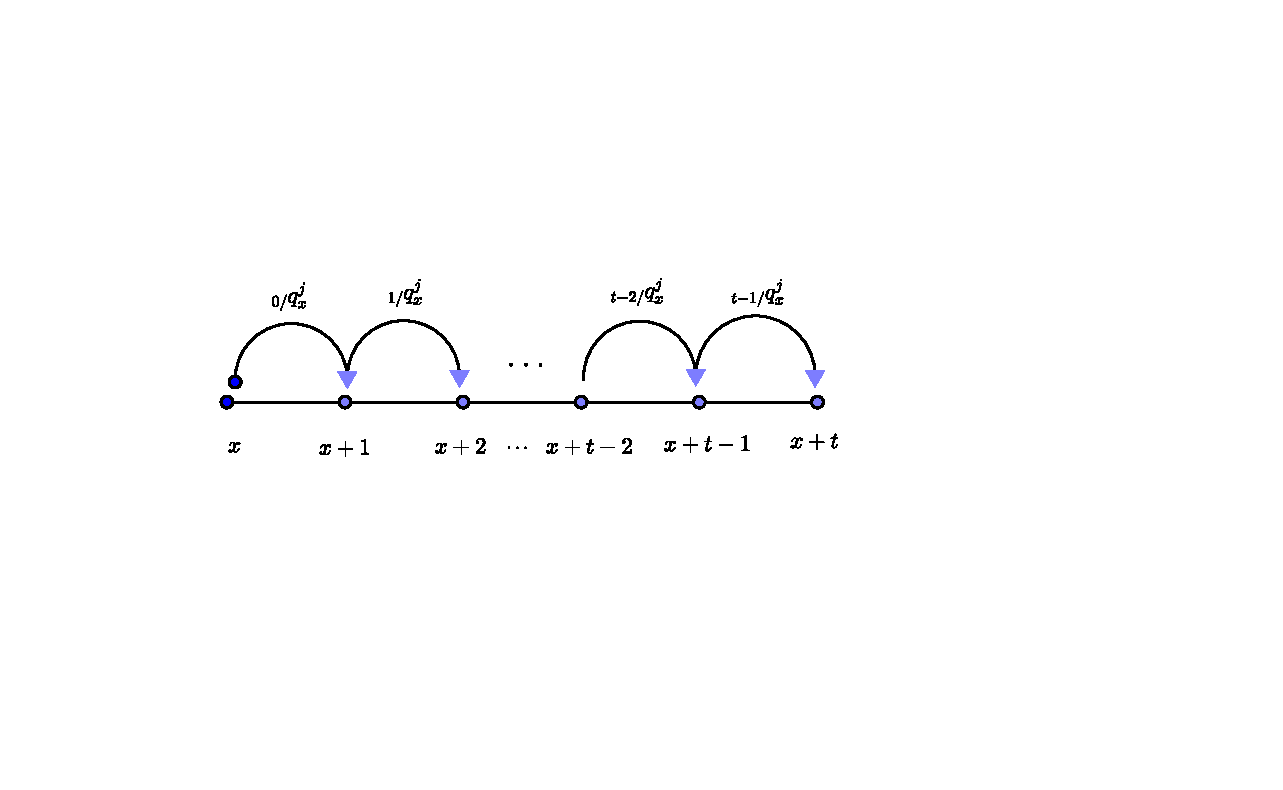
\includegraphics[scale=1.1,trim=70 100 60 100,clip]{tantomort.eps}%left bottom right top
\caption{\centering Explicación de la función biométrica probabilidad diferida de muerte. \\ \textbf{Fuente:} Elaboración propia.}
\label{geog}
\end{figure}

Para dos causas $j$ y $k$ la formulación es sencilla, ya que se ha asumido una denominacón de la mortalidad como una ``partición'' de las posibles causas. Se empezará con la probabilidad de fallecimiento diferida para un individuo con x años cumplidos a la edad de $x+t$ años por las causas $j$ y $k$:

$$
\prescript{}{t/}q_{x}^{jk}=\prescript{}{t/}q_{x}^{j}+\prescript{}{t/}q_{x}^{k}=\frac{d_{x+t}^{j}+d_{x+t}^{k}}{l_{x}}
$$

Entonces se podrá obtener la probabilidad de muerte en los siguientes $t$ años para un individuo de edad $x$ por las causas $j$ y $k$ como suma de los diferidos intermedios:
$$
\prescript{}{t}q_{x}^{jk}=\sum_{i=0}^{t-1}\prescript{}{i/}q_{x}^{jk}=\sum_{i=0}^{t-1}\prescript{}{i/}q_{x}^{j}+\prescript{}{i/}q_{x}^{k}=\frac{\displaystyle\sum_{i=0}^{t-1}\prescript{}{i/}q_{x}^{j}+\sum_{i=0}^{t-1}\prescript{}{i/}q_{x}^{k}}{l_{x}}
$$

se podrá generalizar la probabilidad diferida para un individuo de edad x a la edad x+t para 
Y así pues, se podrá generalizar la probabilidad diferida para un individuo de edad x a la edad x+t para un conjunto $\Lambda=\{j_{1},j_{2},\dots,j_{m}\}\subseteq\Omega$ de causas de mortalidad:

$$
\prescript{}{t/}q_{x}^{\Lambda}=\prescript{}{t/}q_{x}^{j_{1}}+\prescript{}{t/}q_{x}^{j_{2}}\dots\prescript{}{t/}q_{x}^{j_{m}}=\sum_{j\in\Lambda}\prescript{}{t/}q_{x}^{j}=\sum_{j\in\Lambda}\frac{d_{x+t}^{j}}{l_{x}}
$$

Y si se realiza la generalización para la probabilidad temporal de fallecimiento para un individuo de edad $x$ en los próximos $t$ años por una causa incluida en $\Lambda$:

$$
\prescript{}{t}q_{x}^{\Lambda}=\sum_{i=0}^{t-1}\prescript{}{i/}q_{x}^{\Lambda}=\sum_{i=0}^{t-1}\sum_{j\in\Lambda}\prescript{}{i/}q_{x}^{j}=\sum_{j\in\Lambda}\sum_{i=0}^{t-1}\prescript{}{i/}q_{x}^{j}=\sum_{j\in\Lambda}\prescript{}{t}q_{x}^{j}=\sum_{j\in\Lambda}\frac{\displaystyle\sum_{i=0}^{t-1}d_{x+i}^{j}}{l_{x}}
$$

Claramente, en el caso particular en el que se consideran todas las causas, es decir, $\Lambda=\Omega$, se obtienen las siguientes relaciones con las funciones biométricas que no dependen de las causas de mortalidad:

$$
\prescript{}{t/}q_{x}^{\Omega}=\sum_{j\in\Omega}\frac{d_{x+t}^{j}}{l_{x}}=\frac{d_{x+t}}{l_{x}}
$$

\begin{equation}
\prescript{}{t}q_{x}^{\Omega}=\sum_{j\in\Omega}\prescript{}{t}q_{x}^{j}=\prescript{}{t}q_{x}=\frac{l_{x}-l_{x+t}}{l_{x}}
\label{equivcaus}
\end{equation}


\subsection{La dependencia de las causas}

Se ha propuesto un nuevo elemento como función biométrica:
$$
\gamma_{x,j}^{(k)}\equiv \text{Porcentaje de pertenencia a la causa $j$ del fallecimiento $k$ de la cohorte con  edad $x$}
$$
Es decir, se consideran todas las muertes de la cohorte de una edad ordenadas por su ocurrencia, y le se le asocia a cada una un porcentaje  de cada una de las posibles causas consideradas. Esto es, generalizar los conceptos del apartado anterior, ya que antes se consideraba que una muerte sólo podía ser generada por una causa, y en este epígrafe se considera lo contrario.

Así pues, las primeras propiedades de este elemento son:

\begin{equation}
\label{probtot}
\sum_{j\in\Omega}\gamma_{x,j}^{(k)}=1 \,\,\,\,\forall x,k\,\,\,x=0,\dots,\omega\,\,\,k=0,\dots,d_{x}
\end{equation}

\begin{equation}
\label{mortcaus}
d_{x}^{j}=\sum_{i=1}^{d_{x}}\gamma_{x,j}^{(i)}
\end{equation}

\begin{equation}
\label{morti}
d_{x}=\sum_{j\in\Omega}d_{x}^{j}
\end{equation}



Se debe notar ahora que el número de fallecidos por cada causa no tiene que ser entero, sino racional, aunque una vez sumados, debido a la ecuación \ref{probtot}, los fallecidos totales de la edad $x$ de la propiedad \ref{morti} se obtendrán enteros. Veámoslo con un ejemplo:
\vspace{0.3cm}

Suponemos una población ficticia simple. En la edad de 63 años han habido 3 muertes y sólo dos causas, la causa 1 y la causa 2. La tabla de relación de los fallecimientos es la que sigue:

\begin{table}[H]
\centering
\label{ejemplo}
\begin{tabular}{|l|c|c|c|}
\hline
\multicolumn{1}{|c|}{\textbf{$\gamma_{x,j}^{(k)}$}} & \multicolumn{3}{c|}{Muertes} \\ \hline
\multicolumn{1}{|c|}{Edad = 63 años}                     & 1        & 2      & 3        \\ \hline
Causa 1                                          & 0.4      & 0      & 0.9      \\
Causa 2                                         & 0.6      & 1      & 0.1      \\ \hline
\end{tabular}
\end{table}

La propiedad \ref{probtot}, es decir, que cada fallecimiento haya sido correctamente asignado entre todas las posibles causas, se comprueba fácilmente sumando por columnas:
$$
\sum_{j=1}^{2}\gamma_{63,j}^{(k)}=1\,\,\,\forall k=1,2,3
$$

La ecuación \ref{mortcaus} indica las defunciones de cada una de las causas, y se obtiene sumando por filas:
$$
d_{63}^{1}=\sum_{i=1}^{3}\gamma_{63,1}^{i}=0.4+0+0.9=1.3
$$
$$
d_{63}^{2}=\sum_{i=1}^{3}\gamma_{63,2}^{i}=0.6+1+0.1=1.7
$$

Se han obtenido así que los fallecidos por la causa 1 son 1.3 (recordar que en el caso de las causas dependientes no se tienen porqué obtener defunciones por causas enteras), y por la causa 2, 1.7 fallecimientos de individuos de 63 años.

La última ecuación es la de los fallecimientos totales de la población\label{mort}, y se obtiene a partir de la suma de los fallecimientos de todas las causas.  Lógicamente, tendrá que coincidir con el número de muertes indexadas inicialmente en la tabla.

$$
d_{63}=\sum_{j=1}^{2}d_{x}^{j}=1.3+1.7=3
$$

Otro ejemplo más ilustrativo es el caso en el que un portador del SIDA (Síndrome de InmunoDeficiencia Adquirido) de edad 45, el cual se caracteriza por debilitar las defensas del cuerpo humano, sufre un resfriado común y fallece (siendo el fallecido número 110 de este año). La causa que se registra es la de fallecimiento por SIDA, pero ha habido otra causa, el resfriado, que ha influido en el fallecimiento, por lo que una propuesta realizada de porcentajes sería $\gamma_{45,SIDA}^{110}=0.9$ y $\gamma_{45,Resfriado}^{110}=0.1$. Esta propuesta ha sido realizada por el mismo autor del trabajo ya que la causa de mortalidad del SIDA ha sido en gran parte la causante de la muerte, aunque cabe incluir el efecto que ha tenido el resfriado ocurrido en esta defunción ficticia.

Como se ha observado, la desagregación de dependencia de las causas de mortalidad produce un estudio más exhaustivo de las causas, aunque cabe destacar la gran dificultad de toma de tales correlaciones y el sesgo que se produciría. Aún así, los datos obtenidos ajustarían con más precisión la mortalidad y pueden ser agregados para formar la mortalidad total de la población y así poder generar mejores predicciones.
Actualmente en España los partes de defunción indican las diversas causas de fallecimiento aunque sólo acaba indexándose la principal, por lo que no supondría un gran esfuerzo recopilar también el porcentaje de pertenencia de las causas secundarias de muerte, por este mismo motivo, en este trabajo se considerarán las causas independientes, debido a estas restricciones anteriores y el razonamiento de \cite{arnold2015causes}. Aunque no se vaya a utilizar este coeficiente en este trabajo, se ha incluido debido a la importancia que puede tener el estudiar la dependencia entre dos causas y su posible colinealidad para hacer inciso sobre ello.


\subsection{La expresión de la esperanza de vida a partir de las causas de mortalidad}


Si las causas son independientes, la esperanza de vida se puede expresar como:
$$
e_{x}=(\omega-x)-\sum_{j\in\Omega}\sum_{i=0}^{\omega-x-1}(\omega-x-i)\prescript{}{i/}q_{x}^{j}
$$

\begin{dem}\end{dem}
Se sabe que:
$$
e_{x}=\frac{\displaystyle\sum_{i=1}^{\omega-x}l_{x+i}}{l_{x}}=\frac{l_{x+1}+l_{x+2}+\dots + l_{\omega}}{l_{x}}
$$
Si se desbrozan todos los supervivientes como:
$$
d_{x}=l_{x}-l_{x+1}\,\,\,\,\,\,\leadsto \,\,\,\,\,\,l_{x+1}=l_{x}-d_{x}
$$
$$
d_{x+1}=l_{x+1}-l_{x+2}\,\,\,\,\,\,\leadsto \,\,\,\,\,\,l_{x+2}=l_{x+1}-d_{x+1}=l_{x}-d_{x}-d_{x+1}
$$
$$
d_{x+2}=l_{x+2}-l_{x+3}\,\,\,\,\,\,\leadsto \,\,\,\,\,\,l_{x+3}=l_{x+2}-d_{x+2}=l_{x}-d_{x}-d_{x+1}-d_{x+2}
$$
$$
\vdots
$$
$$
l_{x+t}=l_{x}-\sum_{i=0}^{t-1}d_{x+i}
$$

Por tanto se reescribe la esperanza de vida:

$$
e_{x}=\frac{\displaystyle(l_{x}-\sum_{i=0}^{0}d_{x+i})+(l_{x}-\sum_{i=0}^{1}d_{x+i})+\overbrace{\dots}^{\omega-x)}+(l_{x}-\sum_{i=0}^{\omega-x-1}d_{x+i})}{l_{x}}=
$$
$$
=(\omega-x)-\frac{(d_{x})+(d_{x}+d_{x+1})+\overbrace{\dots}^{\omega-x)}+(d_{x}+\dots d_{\omega-x-1})}{l_{x}}=
$$
$$
=(\omega-x)-\frac{(\omega-x)d_{x}+(\omega-x-1)d_{x+1}+\overbrace{\dots}^{\omega-x)}+2d_{\omega-x-2}+d_{\omega-x-1}}{l_{x}}=
$$
$$
=(\omega-x)-\frac{\displaystyle\sum_{i=0}^{\omega-x-1}(\omega-x-i)d_{x+i}}{l_{x}}=(\omega-x)-\sum_{i=0}^{\omega-x-1}(\omega-x-i)\prescript{}{i/}q_{x}=
$$

$$
=(\omega-x)-\sum_{i=0}^{\omega-x-1}(\omega-x-i)\sum_{j\in\Omega}\frac{d_{x+i}^{j}}{l_{x}}=
$$
$$
=(\omega-x)-\sum_{j\in\Omega}\sum_{i=0}^{\omega-x-1}(\omega-x-i)\prescript{}{i/}q_{x}^{j}
$$
\finaldem

Otro método que se puede utilizar es el de caracterizar la esperanza de vida respecto a algunas causas en concreto, es decir, calcular los años esperados que se estima vivir sin fallecer por una (o varias) causas. Esto se obtiene fácilmente a partir de la expresión de la esperanza de vida y con manipulaciones algebraicas sencillas.

Se sabe que la esperanza de vida tiene la siguiente expresión:

$$
e_{x}=\frac{\displaystyle\sum_{i=1}^{\omega-x}l_{x+i}}{l_{x}}=p_{x}+\prescript{}{2}p_{x}+\dots+\prescript{}{\omega-x}p_{x}=\sum_{i=1}^{\omega-x}\prescript{}{i}p_{x}
$$
Por tanto si lo se expresa como tantos de mortalidad por causas quedará:
$$
e_{x}=\sum_{i=1}^{\omega-x}1-\prescript{}{i}q_{x}=\sum_{i=1}^{\omega-x}(1-\sum_{j\in\Omega}\prescript{}{i}q_{x}^{j})=:e_{x}^{\Omega}
$$

Por lo que si se quiere restringir la esperanza de vida a algún grupo de causas o a una única en concreto, esto se realizará modificando el subconjunto de causas que se tome, es decir, estudiarlo para un conjunto de causas $\Lambda\subseteq\Omega$ como:
$$
e_{x}^{\Lambda}=\sum_{i=1}^{\omega-x}(1-\sum_{j\in\Lambda}\prescript{}{i}q_{x}^{j})
$$

Se tendría así otra expresión de la esperanza de vida dependiente de las causas de mortalidad. Esta función se interpreta como los años esperados a vivir siendo el fallecimiento provocado por alguna de las causas incluídas en $\Lambda$. Esta fórmula puede ser de gran utilidad en muchos cálculos actuariales debido a que se puede precisar aún más el cálculo que se realice sobre el asegurado y la tarificación que se le aplique, pudiendo llegar incluso a asegurar (o excluir de un seguro) algunas causas de fallecimiento.
\newpage
\section{Metodología}
Según el INE, la Estadística de Defunciones según la Causa de Muerte constituye una de las fuentes de información más importantes en el campo de la Sanidad.
Las defunciones son consecuencia de un conjunto de causas de tipo biológico, económico, sanitario y social. Por ello, es preciso disponer de información, no sólo del número de fallecimientos que se producen en un país en un determinado período, sino también de todas aquellas circunstancias que rodean el acontecimiento para facilitar la actuación de las Administraciones Sanitarias y del resto de las fuerzas sociales.
Este hecho unido a la escasa disponibilidad de indicadores fiables y exhaustivos para evaluar el nivel de salud de la población, ha motivado que siga incrementándose la demanda de esta estadística, cuyos principales objetivos son los siguientes: 

\begin{enumerate}
\item Proporcionar información sobre la mortalidad atendiendo a la causa básica de la defunción según la CIE, su distribución por grupos de edad, sexo y otras variables de clasificación.
\item Conocer las muertes fetales tardías atendiendo a la causa de la defunción según la CIE.
\item Medir la mortalidad perinatal, proporcionando la base para la obtención de indicadores que permitan evaluar la cobertura y calidad de los servicios sanitarios.
\item Hacer posible la construcción de series históricas para estudiar la evolución de la prevalencia de determinadas causas de defunción, así como otros estudios que satisfagan las necesidades de información que las Administraciones Sanitarias tengan planteadas.
\item Realizar comparaciones territoriales sobre el comportamiento de la mortalidad por grupos de causas de muerte.
\item Suministrar la base para la construcción de indicadores sanitarios recomendados por los Organismos Internacionales.
\end{enumerate}


\subsection{Software y datos}

Para la realización de este trabajo se han utilizado el modelo de Lee-Carter a partir del paquete \emph{demography} \cite{demography} del programa estadístico \emph{R} \cite{rlang}. En esta sección se explicará la metodología utilizada. Adicionalmente, en el anexo se puede encontrar el listado de causas de mortalidad extraído íntegramente.
Es recomendable que junto a la lectura de este trabajo, se visite el repositorio de GitHub \url{https://github.com/JuanJoseVidal/Mortalidad-por-causas.-Desagregaci-n-y-predicci-n.} , en el que se podrán encontrar tanto el código creado y ejecutado, como las tablas de resultados y gráficos obtenidos.


Los datos utilizados han sido extraídos de las siguientes direcciones en la web del INE. Las defunciones por causas se extraen de \url{http://www.ine.es} en la dirección \emph{INEbase / Defunciones según la Causa de Muerte} y la cohorte de supervivientes se toma desde las series históricas de las tablas de mortalidad en la dirección \emph{INEbase / Tablas de mortalidad / Tablas de mortalidad de la población de España. Serie 1975-2015}. Los datos se organizan del siguiente modo:

Las defunciones por causas incluyen las muertes para cada uno de los grupos de causas de mortalidad desde el año 1987 hasta el 2014 y para los grupos de edad de 0 a 1 años, de 1 a 4 años y grupos de edad de 5 años (5-9, 10-14, 15-19, \dots) hasta llegar a 95 o más años, donde se agrupa toda la cola restante. Se ha comprobado que la suma de estas causas resulta exactamente la mortalidad total que se puede obtener de las tablas de mortalidad también descargadas. 


Queda claro que la modelización de la mortalidad supone una importante labor en el desarrollo demográfico de un estado, ya que facilita la comprensión de su evolución y permite actuaciones preventivas debido a que identifica posibles carencias poblacionales.

\subsection{Métodos de clasificación}
A continuación se introducirán los dos grandes tipos de algoritmos que utiliza todo estadístico como herramienta de clasificación, los métodos supervisados y no supervisados. Dentro de éstos últimos se encuentra el clustering, que será el método que más se profundizará, ya que es el que se utilizará en la parte práctica del trabajo.

\subsection*{La classificación supervisada}
El aprendizaje supervisado recoje todas aquellas técnicas los objetivos de las cuales es inferir una función o regla de decisión a partir de lo que se conoce como conjunto de entrenamiento. En este problema de clasificación se tiene un conocimiento a priori de objetos ya etiquetados para la tarea de clasificar de nuevo.
El problema se divide en dos fases:
\begin{enumerate}
\item En la primera se dispone de un conjunto de entrenamiento a partir del cual se construye un modelo para clasificar. Es habitual que el conjunto de entrenamiento se divida en dos, tomando un porcentaje de los datos para validar y optimizar el clasificador.
\item En la segunda fase se aplica el modelo obtenido para determinar la categoria de cada nuevo dato.
\end{enumerate}

El problema de la clasificación supervisada ha sido abordado desde distintos enfoques. Se pueden encontrar algoritmos basados en las distancias a los elementos de cada clase, como es el clásico \emph{k-means} o el \emph{knn} (del inglés \emph{k-nearest neighborhoods}). Estos métodos son los denominados no paramétricos \cite{coha}. Los también muy extendidos son los paramétricos o de máxima probabilidad, que basan sus reglas de clasificación discriminante en las funciones de distribución de los datos de entrenamiento \cite{deki}.

Una de las metodologías con mayor aplicación en los últimos tiempos son las denominadas \emph{Support Vector Machines} (SVM), que son un conjunto de algoritmos que han proporcionado muy buenos resultados en problemas reales de Machine Learning. Aunque la clasificación supervisada tiene un gran interés actual, este trabajo se centrará en la clasificación no supervisada.



\subsection*{La clasificación no supervisada}

Citando el clásico libro de Kaufman i Rousseeuw titulado \emph{Finding groups in data} \cite{fgd}, se puede decir que \emph{El análisi cluster es el arte de encontrar grupos en los datos}.

También conocido como clasificación no supervisada o análisis de conglomerados, el cústering tiene como finalidad dividir un conjunto de objetos en grupos, de forma que los perfiles de los objetos que pertenecen a un mismo grupo sean similares entre sí, mientras que respecto a los otros sean distintos.

Para este tipo de clasificación no se tiene ningún conocimiento a priori, lo que dificulta el problema y, de hecho, después de clasificar se tendrá que incluir un costoso proceso de interpretación y validación de los grupos obtenidos. Realizar una interpretación de la clasificación obtenida por un método de clustering requiere, en primer lugar, un conocimiento suficiente del problema analizado, a parte de estar abierto a la posibilidad de que no todos los grupos sean interpretables.

La actividad usual de clasificación no supervisada de un conjunto de objetos consta de los siguientes pasos \cite{jandub88}:

\begin{itemize}
\item Representación de los objetos incluyendo opcionalmente la extracción de características y/o selección.
\item Definición de la medida de proximidad de los objetos al dominio de los datos.
\item Clustering y agrupación.
\item Abstracción de los datos, si es necesario.
\item Valoración de los outputs.
\end{itemize}

La representación de los objetos hace referencia al número de clases, el número de objetos disponibles, y el nombre, tipo y escala de las características de un algoritmo de clustering. La selección de características es el proceso para identificar el subconjunto más efectivo de atributos originales para utilizar al clustering. La extracción de características es la utilización de una o más transformaciones del input para producir de nuevas. Ambas técnicas pueden ser utilizadas para obtener un conjunto apropiado de características para utilizar. La proximidad de objetos es usualmente medida con una función llamada disimilaridad que más adelante se explicarán.

El paso de agrupación puede ser realizado de distintas maneras. El clustering de los outputs puede ser fuerte, en el que se realice una partición de los datos en grupos, o difuso, donde cada objeto tiene un grado de pertenencia a cada cluster del output. Existen dos tipos de métodos de clustering, los algoritmos de clustering jerárquicos, que producen una serie de particiones basadas en un criterio para combinar o separar clusters basados en la similaridad, y los algoritmos de clustering particionales, que identifican un subconjunto que resuelve usualmente un criterio de optimización.

La abstracción de datos es el proceso de extraer representaciones simples y compactas del conjunto de objetos. La valoración de un output del procedimiento de clustering tiene muchas facetas. Una es actualmete la evaluación del dominio de los dates frente a la del algoritmo del clustering utilizado. El estudio de la tendencia al clustering, donde los inputs de los datos son examinados para ver si hay algún mérito en realizar el análisi por clusters a priori de que sea procesado, es una investigación relativamente inactiva en esta área, y no estará considerada en este trabajo. El lector interesado puede tomar referencias en \cite{dub87} y \cite{che} para más información.

La validez del análisi por clusters, por contrario, es la valoración del output del procedimiento. Utiliza un criterio específico de optimización, aunque puede llegar incluso a la subjetividad \cite{dub93}.





\subsection{El clustering como método de clasificación}

El clustering es una técnica de análisis multivariante no supervisada que tiene como objetivo organizar un conjunto de datos a partir de sus distancias. El análisis por clusters es la organización de objetos, usualmente representados como vectores de medidas, o puntos en un espacio multidimensional, en conjuntos basados en la similaridad. Intuitivamente, los objetos de un cluster son más similares entre ellos que con los de otro. La variedad de técnicas para representar los datos, medir proximidades entre distintos elementos y agrupar los datos ha producido un amplio repertorio de métodos de clasificación no supervisada.

Se definirá primero el concepto de disimilaridad:
\begin{defi} Disimilaridad \end{defi}
Sea $\mathscr{X}$ un conjunto de objetos, y sea la aplicación:
$$
\mathfrak{d}:\mathscr{X}\times\mathscr{X}\longrightarrow \mathds{R}
$$
$$
(\mathbf{x}_{i},\mathbf{x}_{j})\longmapsto \mathfrak{d}(\mathbf{x}_{i},\mathbf{x}_{j})
$$
que se llamará disimilaridad si cumple las siguientes propiedades:
\begin{description}
\item[(D1)] $\mathfrak{d}(\mathbf{x}_{i},\mathbf{x}_{j})\geq 0\,\,\,\, \forall i,j\in \{1,\dots,d\}$  (Definida positiva)
\item[(D2)] $\mathfrak{d}(\mathbf{x}_{i},\mathbf{x}_{j})=0\longleftrightarrow \,\, \mathbf{x}_{i}=\mathbf{x}_{j}\,\, \forall i,j\in \{1,\dots,d\}$
\item[(D3)] $\mathfrak{d}(\mathbf{x}_{i},\mathbf{x}_{j})=\mathfrak{d}(\mathbf{x}_{j},\mathbf{x}_{i})\,\,\,\, \forall i,j\in \{1,\dots,d\}$  (Simetría)
\end{description}

Se observa que si se le añade una condición:
\begin{description}
\item[(D4)] $\mathfrak{d}(\mathbf{x}_{i},\mathbf{x}_{j})\leq \mathfrak{d}(\mathbf{x}_{i},\mathbf{x}_{k})+\mathfrak{d}(\mathbf{x}_{k},\mathbf{x}_{j}) \,\,\,\, \forall i,j,k\in \{1,\dots,d\}$
\end{description}
se tendrá la definición formal de distancia, aunque no es utilizada en las técnicas de clasificación no supervisada. 

Se puede entender así, que cuando más grande sea $\mathfrak{d}(\mathbf{x}_{i},\mathbf{x}_{j})$, mayor será la ``diferencia''/disimilaridad entre los objetos $\mathbf{x}_{i}$ i $\mathbf{x}_{j}$, es decir, presentan menos similitud.

\begin{exem}
\end{exem}

Se define el coeficiente de correlación de Pearson entre $f$ y $g$ como:
$$
R(f,g)=\frac{\sum_{i=1}^{n}(x_{if}-m_{f})(x_{ig}-m_{g})}{\sqrt{\sum_{i=1}^{n}(x_{if}-m_{f})^{2}}\sqrt{\sum_{i=1}^{n}(x_{ig}-m_{g})^{2}}}
$$
donde las $x_{ij}$ el elemento de la matriz de datos que representa la variable $j$ de la observación $i$, y las $m_{f}$ la medias de todos los valores para la variable $f$.

Entonces a partir de aquí se podrá generar la siguiente disimilaridad:
$$
d(f,g)=\frac{1-R(f,g)}{2}
$$

El algoritmo que se utilizará es el PAM (Partitioning Around Medoids), en el que se van seleccionando elementos de los datos iniciales como centro de los clusters (medoides) y se van agrupando los datos a partir de modelos de optimización lineal.

\vspace{0.5cm}


El clustering es una técnica de mucha utilidad en la exploración de análisis de patrones, agrupaciones, toma de decisiones y aprendizaje automático (machine learning), minería de datos, recuperación de documentos, segmentación de imágenes y detección de datos anómalos.

\subsection*{El algoritmo PAM}

Se pasa ahora a resumir brevemente como funciona este algoritmo, que se utilizará en la parte práctica. Si se desean más detalles se sugiere la consulta de \cite{fgd}.

\begin{itemize}
\item En la fase de construcción, el algoritmo comienza con la búsqueda de un número $k$, previamente especificado, de objetos representativos o medoides entre las observaciones del conjunto de datos. Utilizando la matriz de disimilaridades, se asigna cada objeto a su medoide más cercano. Esta matriz puede darse como un input o calcularse si se le introduce la disimilaridad a utilizar.
\item En la fase de intercambio se modifica el conjunto de objetos representativos con el fin de mejorar la partición a la que da lugar. Esto se realiza considerando todos los pares de objetos $(i,h)$ para los que el objeto $i$ había sido seleccionado como un medoide mientras que el objeto $h$ no. Se determina el efecto que tiene llevar a cabo el intercambio, es decir, seleccionar $h$ en vez de $i$. Este efecto se mide en términos de la suma de disimilaridades entre cada objeto y el objeto representativo más similar a él. Cuando se encuentra un mínimo local de ésta función objetivo el algoritmo se detiene.
\end{itemize}

Cuando se construyen particiones con un gran número fijo de $k$ clusters, se asume que existe una función la cual mide la calidad de distintos clusterings finales, donde el objetivo es minimizar la distancia total entre los objetos.

El algoritmo está basado en dos decisiones las cuales derivan en un modelo a resolver. La primera es definir para un conjunto de $n$ objetos $x_{i}$, un vector $y_{i}$ de variables binarias la cual sea 1 cuando el objeto $x_{i}$ sea representativo y 0 en caso contrario. A la segunda, para cada objeto $x_{j}$ se le asignará una variable $z_{ij}$ binaria la cual será 1 si y sólo si el objeto $j$ es asignado al cluster donde $x_{i}$ es el objeto representativo. Cabe recordar que PAM es un algoritmo de clustering fuerte, por lo que un elemento sólo podrá pertenecer a un único cluster.

Así, el modelo que se tendrá que resolver será el siguiente:
$$
minimizar\sum_{i=1}^{n}\sum_{j=1}^{n}d(x_{i},x_{j})z_{ij}
$$
sujeto a:

$$
\sum_{i=1}^{n}z_{ij}=1, \hspace*{0.5 cm} j=1,2,\dots,n
$$

$$
z_{ij}\leq y_{i}, \hspace*{0.5 cm} i,j=1,2,\dots,n
$$

$$
\sum_{i=1}^{n}y_{i}=k, \hspace*{0.5 cm} k=\text{número prefijado de clusters}
$$

$$
y_{i},\,z_{ij}\in\{0,1\} , \hspace*{0.5 cm} i,j=1,2,\dots,n
$$

Usualmente no se conoce el número de clusters óptimos de un conjunto de datos, así que el trabajo de optimización ha de ser complementado con la ejecución de éste para distintos valores $k$. Una manera posible de seleccionar este valor es mediante las siluetas que se explicarán a continuación.

\subsection{Silueta y silueta media}

Los conceptos de \emph{silueta} y \emph{silueta media}, así como su representación gráfica, son muy útiles para la evaluación de la clasificación de un método de clustering. \emph{Kaufman i Rousseeuw} \cite{fgd} son una referencia básica para la descripción de estos conceptos.

\begin{defi}Silueta
\end{defi}

La silueta de la i-ésima observación, que se denotará por $s(i)$, se calcula como:
$$
s(i)=\frac{b(i)-a(i)}{max\{a(i),b(i)\}}
$$
siendo $a(i)$ la disimilaridad media entre la observación $i$ y todas las otras que pertenecen al mismo grupo en el que está $i$, y $b(i)$ es la disimilaridad media entre $i$ y el cluster vecino, es decir, el más cercano según la distancia definida sin ser él mismo.

Queda claro que los valores con una $s(i)$ grande están bien situados en su grupo. Que $s(i)$ se acerque a 0 indica que la observación está cercana a dos clusters, y si el valor es negativo es que probablemente estén situados en el cluster equivocado.

Un ejemplo puede ser el siguiente:

\begin{figure}[H]
\centering
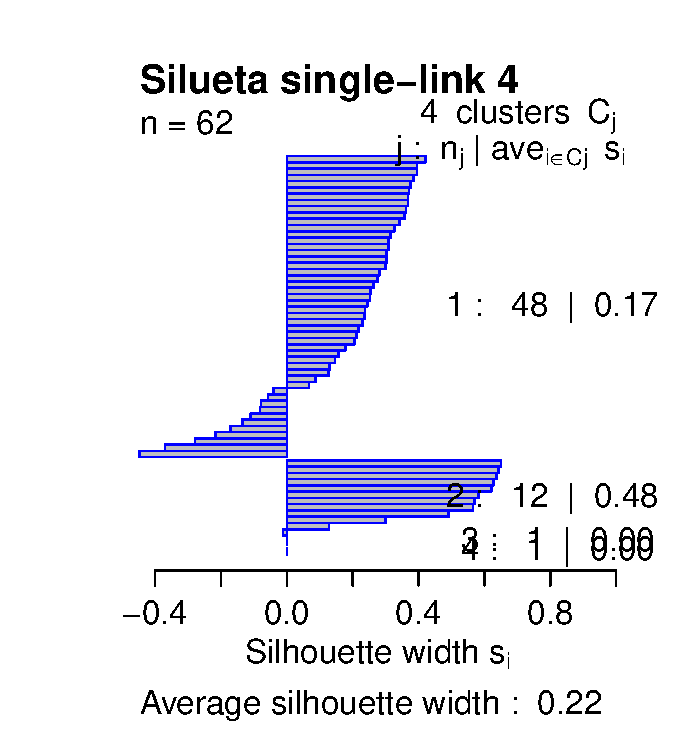
\includegraphics[scale=0.6]{silueta.eps}
\caption{\centering Silueta de un procedimiento de clustering \\ \textbf{Fuente:} Elaboración propia para otro trabajo.}
\end{figure}

Donde se observa como se le asocia una silueta a cada elemento y se observa su pertenencia al cluster al que se ha incluido a partir de sus siluetas medias..
\begin{defi} Silueta media
\end{defi}

La media de los valores de $s(i)$ para todos los objetos de un cluster recibe el nombre de amplitud mediana de la silueta de dicho cluster y se obtiene teniendo en cuenta el conjunto de datos, es decir $\sum_{i \in Cluster}\frac{s(i)}{n}$.

La amplitud media de la silueta varía entre -1 y 1 y ha sido utilizada tanto como para evaluar la calidad de una clasificación como para estimar el número correcto de grupos: la partición con mayor amplitud media de la silueta se toma como partición óptima.


Kaufmann i Rousseeuw nombraron este máximo como \emph{silhouette coefficient} y daron interpretaciones subjetivas a su valor. Estas interpretaciones son: si pertenece al intervalo $[0.71,1]$ es una estructura \emph{fuerte}, si pertenece al intervalo $[0.51,0.70]$, la partición es \emph{razonable}, mientras que si los valores son inferiores a $0.51$, se sugiere que la estructura encontrada es \emph{débil}.


Se introducirá ahora el modelo de mortalidad que se utilizará para modelizar las causas, el modelo de Lee-Carter.

\subsection{El modelo de Lee-Carter}

El modelo de Lee-Carter ha sido muy utilizado desde su publicación en 1992 \cite{lee1992modeling}. Ronald D. Lee and Lawrence R. Carter proponen un modelo basado en una variación de trabajos previos \cite{bozik1989time} \cite{lederman2012classification}. El modelo tiene dos factores, edad y tiempo. Más específicamente, utiliza el método de descomposición en valores singulares para extraer los parámetros específicos de la edad  así como el correspondiente al índice de variación en el tiempo, que se ajusta reajustando el número total de muertes observadas. Dos puntos fuertes del modelo son su simplicidad y su robustez para las tasas de mortalidad, ya que produce resultados equilibrados, a parte de que se puede diferenciar claramente los elementos que dependen de la edad y los que dependen del año.

El objetivo de comprender la dinámica de la mortalidad, bajo la perspectiva demográfica, se basaba únicamente en estudios lineales a partir de la edad y la información conocida, lo cual generaba sobre-estimaciones e información inexacta. Lo anterior no permitía un análisis muy profundo en términos de actuaría de seguros y pensiones. Los estudios de este tipo iniciaron con  modelos  deterministicos  como  el  de  Gompertz  en  1825 el  cual  presenta una estimación satisfactoria de la mortalidad, sin embargo, sobreestima el indicador para  edades  superiores  a  80  años.  El  modelo  de  Heligman  y Pollard (1980) continuó avanzando en el tema, para lo cual, a partir de interpolaciones, dio pasos iniciales hacia el objetivo de proyección de mortalidad en aras de estructurar los estudios actuariales que sustentan los negocios de seguros y pensiones. En los años recientes las tendencia se ha inclinado hacia el modelo estocástico presentado por Lee y Carter \cite{lee1992modeling}. 

Desde entonces, este modelo ha sido utilizado para aplicaciones demográficas y actuariales en todo el mundo. El modelo de Lee-Carter concebido para pronosticar mortalidad y analizar su dinámica fue definido en 1992, su intención más allá de analizar la interacción entre variables como tasa de mortalidad, esperanza de vida e índice de mortalidad se limita por los patrones existentes en esta temática, es decir, no incluye información relativa a la accidentalidad, avances en medicina, guerras u otros eventos que pueden marcar un punto de inflexión. El modelo basa su aproximación en la proyección de la tendencia histórica presentada por las variables, así mismo, su composición probabilistica permite, a través de series de tiempo, generar análisis sobre el comportamiento futuro como lo pueden ser pronósticos e intervalos de confianza. A pesar de  sus  limitantes,  la  aproximación  definida  por  Lee  y  Carter  en  este  sentido  es  utilizada ampliamente en el medio demográfico y logra estar presente en un gran porcentaje de las investigaciones sobre el tema.

La diferenciación más importante presentada por Lee y Carter en su artículo fue la incorporación  de  la  información  en  dos  dimensiones,  es  decir,  mortalidad  a  través  de  periodos de tiempo. Concretamente, el modelo asume que la dinámica de mortalidad responde a un parámetro generado por la regresión: el índice de mortalidad. A partir de este índice se puede proyectar el comportamiento de la mortalidad usando un modelo clásico de series de tiempo como lo es Box - Jenkins, ver  \cite{lee1992modeling}. De forma similar el modelo permite definir conclusiones sobre la esperanza de vida y tablas de mortalidad.

\vspace{0.5cm}

En particular, el modelo de Lee-Carter trata de estimar $m_{x,t}$, la tasa central de mortalidad, para la edad $x$ y el año $t$. El modelo ajusta la matriz de tasas de mortalidad siguiendo la expresión:

\begin{equation}
\label{leecarter}
log(m_{x,t})=a_{x}+b_{x}k_{t}+\varepsilon_{x,t}
\end{equation}

Las $a_{x}$ recogen el efecto en la mortalidad (log-mortalidad) exclusivo de la edad, las $b_{x}$ son las constantes respecto a la edad indicando qué tasas decrecen más lentamente en respuesta a los cambios y la variación del tiempo. $k_{t}$ son los índices de variación en el tiempo del nivel de mortalidad, y los $\varepsilon_{x,t}$, que tratan de recoger las mejoras (o empeoramientos) de la mortalidad debido al momento en el que se tomó cada $m_{x,t}$ y son los términos correspondientes a las fluctuaciones aleatorias con esperanza 0 y varianza $\sigma^{2}_{x,t}$ que describen las influencias no capturadas por el modelo. El modelo no proporciona una solución única, por lo que se le añaden dos restricciones: $\sum_{x}b_{x}=1$
 y $\sum_{t}k_{t}=0$.

\subsection{Los modelos ARIMA}

Principalmente, se definen los procesos ARIMA se necesitará primero definir los subprocesos que lo componen. Primero se deinirán los procesos aleatorios puros o ruido blanco, AP. Se denotan como $Y_{t}=\varepsylon_{t}$, y satisfacen las siguientes propiedades:
$$
E[\varepsilon_{t}]=0\,\,\,\, \forall t
$$
$$
Var[\varepsilon_{t}]=E[\varepsilon_{t}]=\sigma^{2} \,\,\,\, \forall t
$$
$$
Cov[\varepsilon_{t},\varepsilon'_{t}]=E[\varepsilon_{t}\varepsilon'_{t}]=\sigma^{2} \,\,\,\, t\neq t'
$$

Seguidamente se definen los procesos autorregresivos de orden $p$, AR(p), definidos como:
$$
Y_{t}=\phi_{1}Y_{t-1}+\phi_{2}Y_{t-2}+\dots+\phi_{p}Y_{t-p}+\varepsilon_{t}
$$

donde p denota el retardo máximo, las $\phi_{i}$ son los parámetros del modelo, y $\varepsilon_{t}$ denota un proceso aleatorio puro.

\vspace{0.3cm}

Seguidamente se definen los procesos autorregresivos de medias móviles de orden $q$, MA(q), como una combinación lineal de procesos aleatorios puros:
$$
Y_{t}=\varepsilon_{t}-\theta_{1}\varepsilon_{t-1}-\theta_{2}\varepsilon_{t-2}-\dots-\theta_{q}\varepsilon_{t-q}
$$

\vspace{0.3cm}

Un proceso de tipo ARMA(p,q) está formado por un AR(p) y un MA(q):
$$
Y_{t}=\phi_{1}Y_{t-1}+\phi_{2}Y_{t-2}+\dots+\phi_{p}Y_{t-p}+\varepsilon_{t}-\theta_{1}\varepsilon_{t-1}-\theta_{2}\varepsilon_{t-2}-\dots-\theta_{q}\varepsilon_{t-q}
$$

Además, cuando no se tiene un proceso estacionario, existen transformaciones que lo convierten en estacionario. Por ejemplo a través de difrencias de orden 1, 2, \dots .
\vspace{0.3cm}

Así pues, se definirá un proceso $Y_{t}$ como ARIMA(p,d,q), si al tomar las diferencias de orden d se obtiene un proceso de tipo ARMA(p,q). 

Estos modelos son usualmente utilizados en la modelización de series temporales para realizar extrapolaciones de los datos, lo cuál se comprobará en la parte práctica cuando se realice la predicción de los tantos de mortalidad para los grupos de causas de mortalidad creados.

\newpage
\section{La mortalidad por causas}

En esta sección se introducen los datos obtenidos de las defunciones de las causas y estudiar su distribución. Lo primero que se propone es observar cómo ha evolucionado la mortalidad en el periodo 1987-2014.

\begin{figure}[H]
\centering
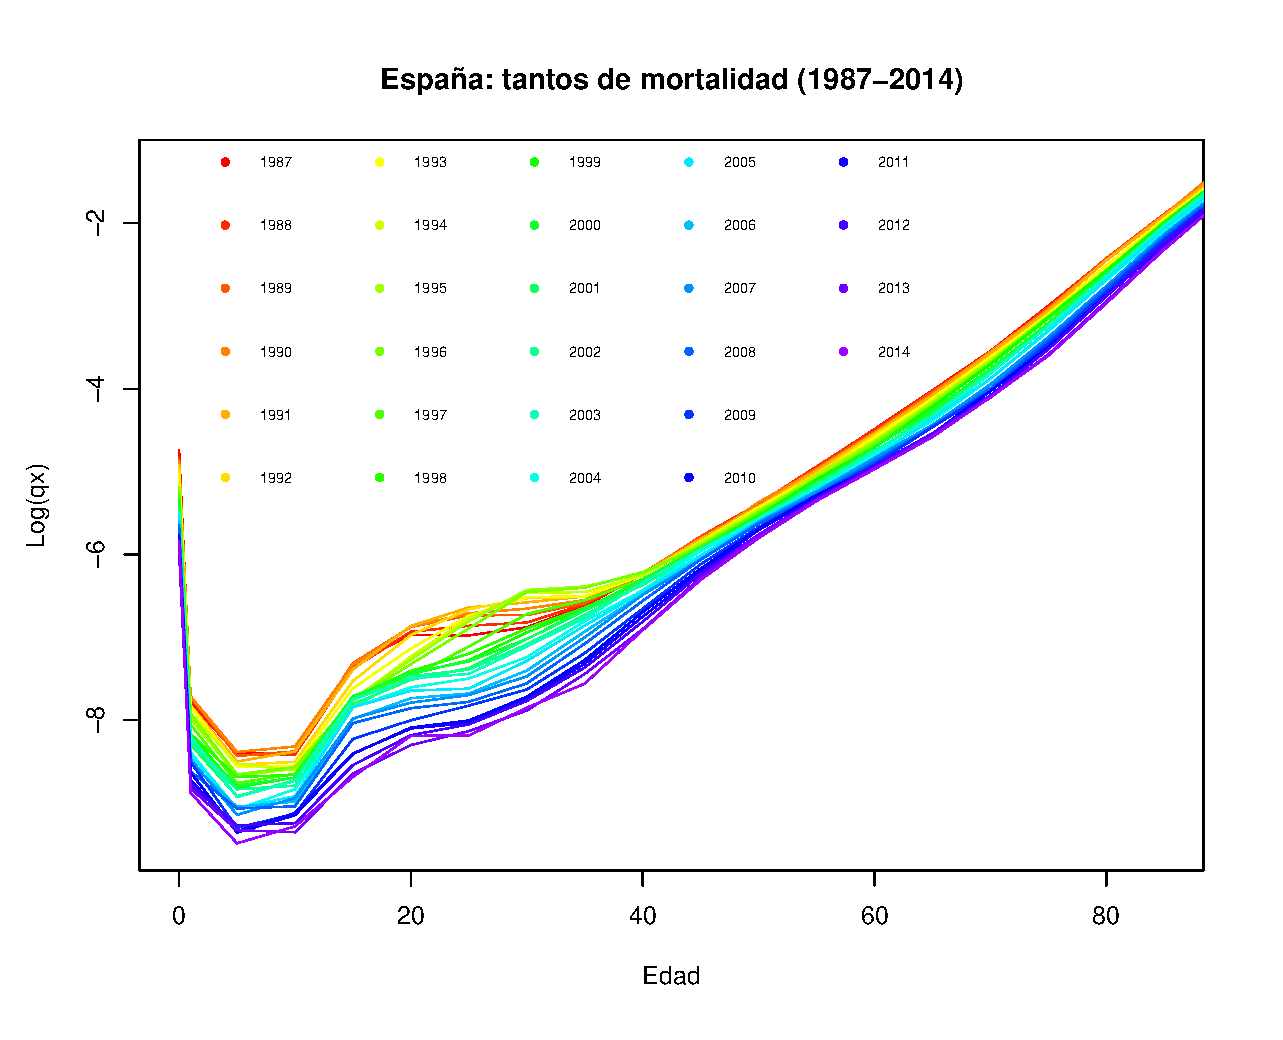
\includegraphics[scale=0.7]{qxtotal.eps}
\caption{\centering Evolución de la mortalidad española desde 1987 hasta 2014. \\ \textbf{Fuente:} Elaboración propia a partir de datos de INE.}
\label{qxtot}
\end{figure}

La mortalidad se ha ido reduciendo progresivamente a lo largo del tiempo como se puede observar en la figura \ref{qxtot}. Se puede observar como para las edades comprendidas entre 20 y 40 años no se ha producido este fenómeno, aunque ya que este crecimiento aparece en los años 90, se puede suponer que es debido al aumento de accidentes de tráfico y de enfermedades de transmisión sexual. Cabe destacar otro punto importante de este gráfico: el gran descenso que aparece de 0 a 1 años, que como ya se sabe, la época de adaptación al medio es una edad crítica en la supervivencia humana.



\vspace{0.3cm}

Por lo que respecta a las causas de la mortalidad, los datos se estructuran en 17 grupos causales, separados en 27 grupos de edad (0-1 años, 1-4 años, 5-9 años,\dots) para los años desde el 1987 hasta el 2014, por lo que se considerarán 17 matrices de $21\times 27$ elementos, los cuales son valores enteros positivos que representan las defunciones, siendo las filas el grupo de edad al que pertenecen y en las columnas el año de ocurrencia, y cada matriz la correspondiente a cada causa.


\begin{table}[H]
\centering
\begin{tabular}{l|l}

 Número & Nombre completo \\ 
  \hline
Grupo causal 1 & 001-008  I.Enfermedades infecciosas y parasitarias (1) \\ 
 Grupo causal 2 & 009-041  II.Tumores \\ 
 Grupo causal 3 & 042-043  III.Enfermedades de la sangre y de los órganos hematopoyéticos,\\
 &	 y ciertos trastornos que afectan al mecanismo de la inmunidad \\ 
Grupo causal 4 & 044-045  IV.Enfermedades endocrinas, nutricionales y metabólicas \\ 
Grupo causal 5 & 046-049  V.Trastornos mentales y del comportamiento \\ 
Grupo causal 6 & 050-052  VI-VIII.Enfermedades del sistema nervioso y de los órganos de los sentidos \\ 
Grupo causal 7 & 053-061 IX.Enfermedades del sistema circulatorio \\ 
Grupo causal 8 & 062-067  X.Enfermedades del sistema respiratorio \\ 
Grupo causal 9 & 068-072  XI.Enfermedades del sistema digestivo \\ 
Grupo causal 10 & 073  XII.Enfermedades de la piel y del tejido subcutáneo \\ 
Grupo causal 11 & 074-076  XIII.Enfermedades del sistema osteomuscular y del tejido conjuntivo \\ 
Grupo causal 12 & 077-080  XIV.Enfermedades del sistema genitourinario \\ 
Grupo causal 13 & 081  XV.Embarazo, parto y puerperio \\ 
Grupo causal 14 & 082  XVI.Afecciones originadas en el periodo perinatal \\ 
Grupo causal 15 & 083-085  XVII.Malformaciones congénitas, deformidades y anomalías cromosómicas \\ 
Grupo causal 16 & 086-089  XVIII.Síntomas, signos y hallazgos anormales clínicos y de laboratorio,\\
& no clasificados en otra parte (2) \\ 
Grupo causal 17 & 090-102  XX.Causas externas de mortalidad \\ 

\end{tabular}
\caption{\centering Relación utilizada en el trabajo de número de causa y causa real.  \\ \textbf{Fuente:} Instituto Nacional de Estadística (INE).}
\label{causmean}
\end{table}

El anexo contiene el listado completo de causas de mortalidad según la clasificación internacional CIE-10, así como su correspondencia con la nomenclatura anterior, CIE-9. Lo primero que se representará es la distribución de las defunciones que se presenta en 2014 para toda España con el ánimo de conseguir una visión más clara de cuáles son las causas de mortalidad más comunes:

\begin{figure}[H]
\centering
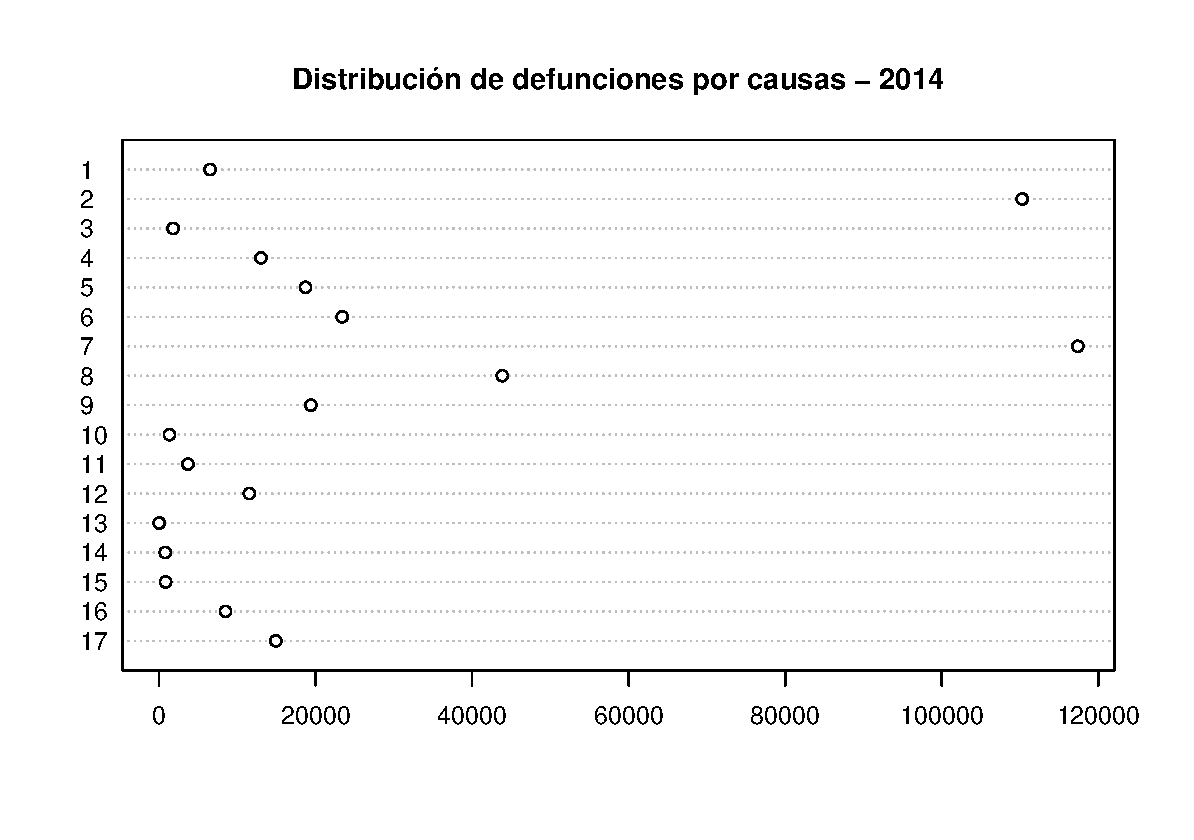
\includegraphics[scale=0.4]{distrcaus.eps}
\caption{\centering Distribución de las defunciones por causas en 2014. \\ \textbf{Fuente:} Elaboración propia a partir de datos de INE.}
\label{distrcaus}
\end{figure}

Se observa en la figura \ref{distrcaus} como la causa 2, tumores, y la causa 7, enfermedades del sistema circulatorio, se diferencian respecto al resto en el tamaño de defunciones que les pertenecen. Para poder estudiar con mejor detalle cuáles son las diferencias que presentan, se incluye a continuación un diagrama de caja y bigotes según el tamaño de las causas al igual que una distribución de las defunciones menos comunes:


\begin{figure}[H]
 \centering
  \subfloat[\centering Diagrama de bigotes y cajas para las causas de mortalidad.]{
   \label{boxplotcaus}
    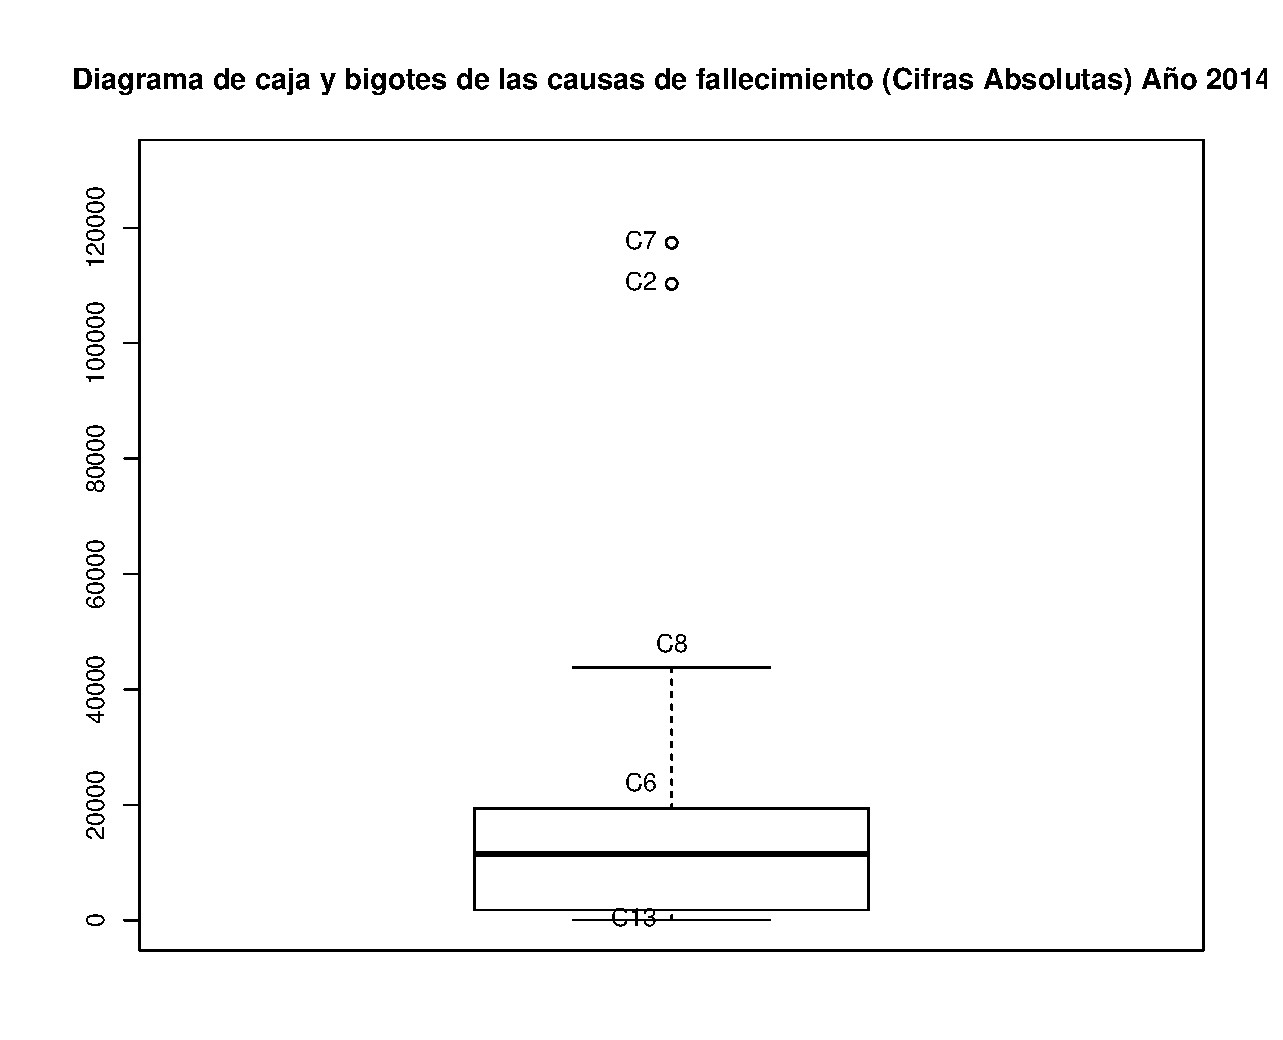
\includegraphics[width=0.55\textwidth]{boxplot.eps}}
  \subfloat[\centering Distribución de las causas de mortalidad (excepto la 2 y la 7).]{
   \label{distrcaus2}
    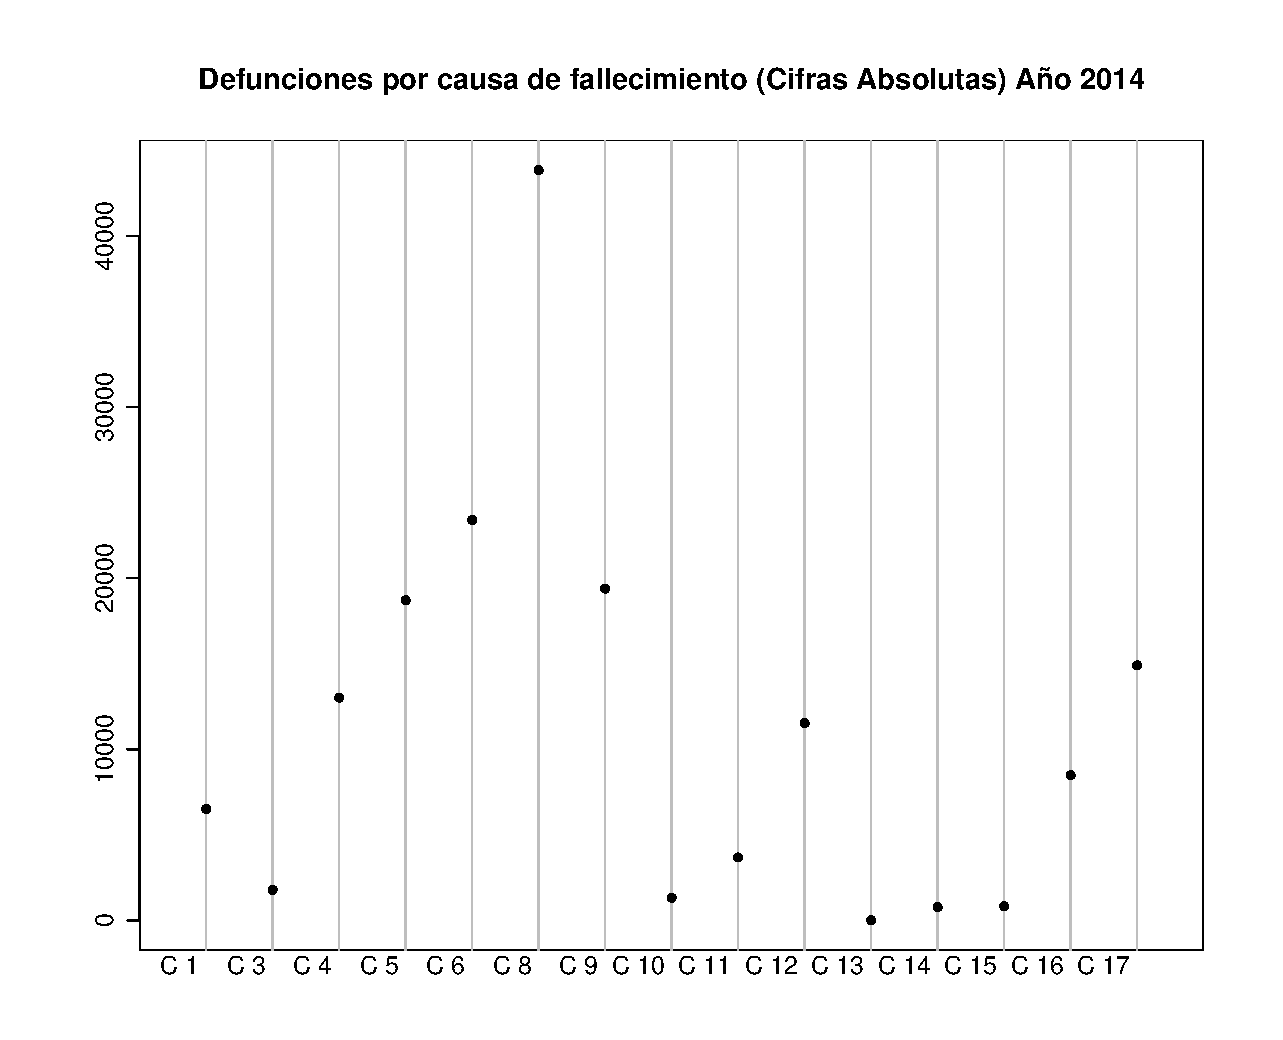
\includegraphics[width=0.55\textwidth]{distrcaus2.eps}}
 \caption{\centering Distribución de las defunciones por causas menos comunes en 2014. \\ \textbf{Fuente:} Elaboración propia a partir de datos de INE.}
 \label{f:animales}
\end{figure}


No era de extrañar que, como se observa en la figura \ref{boxplotcaus}, tanto la cuantía de defunciones de la causa 2 y de la causa 7 tienen valores anómalos respecto a todas las otras en cuanto a cuantía se refiere, que coincide con lo que se había observado en la figura \ref{distrcaus}. 
Se observa también que las causas más relevantes, después de las dos nombradas anteriormente, son la causa 8, enfermedades del sistema respiratorio, la causa 6, enfermedades del sistema nervioso y de los órganos de los sentidos, junto con la causa 5, trastornos mentales y del comportamiento, y la causa 9, enfermedades del sistema digestivo.

Ya que el objetivo de este trabajo es modelizar las causas de mortalidad por separado y, debido a que existen varias causas con un número pequeño de muestras, se ha propuesto la agregación de los datos para estudiar conjuntamente diversas causas y poder obtener modelos más estables que los que se obtendrían con pocos datos. Así pues, se ha decidido agrupar por evolución histórica, ya que lo que se pretende es predecir la evolución futura de las causas.

\newpage
\section{Resultados}

En este apartado se presentan los resultados obtenidos a lo largo del estudio, así como la intuición que nos ha llevado a realizarlos, con ellos daremos respuesta a los interrogantes planteados inicialmente. 
\subsection{Correlación y agrupación de las causas de mortalidad}

Inicialmente se presentará un mapa de calor de la matriz de correlaciones de las causas de mortalidad, donde ya se observarán distintos posibles grupos y lo que reforzará un escalado multidimensional. Seguidamente se representará a partir de dos componentes principales las agrupaciones obtenidas con el algoritmo PAM para 3, 4 y 5 clusters y, con el soporte de la silueta media y de distintos dendrogramas, concluiremos que el número final de clusters será 4 y cuáles serán los elementos que pertenecerán a cada agrupación.

Como se ha indicado, para empezar a estudiar la similitud de la evolución de las causas de mortalidad se requerirá de una matriz de correlación o matriz de similitudes entre las causas dependiente de la evolución de la mortalidad que han presentado durante todos los años, sobre la que se aplicara el algoritmo PAM explicado anteriormente. Al estudiar cómo han evolucionado respectivamente a lo largo del tiempo, se ha representado la matriz de correlaciones como mapa de calor para poder observar mejor los valores obtenidos.

\begin{figure}[H]
\centering
\includegraphics[scale=0.7]{corrplot.eps}
\caption{\centering Mapa de calor de la matriz de correlación entre las causas de mortalidad. \\ \textbf{Fuente:} Elaboración propia.}
\label{mapacalor}
\end{figure}


Se observa en la figura \ref{mapacalor} que las causas 1, 13 y 16 tienen una correlación prácticamente nula con todos los otros elementos; las causas 7, 14, 15 y 17 presentan una correlación negativa con la gran mayoría de las otras causas, y los elementos del 2 al 6 y del 8 al 12 presentan una correlación positiva entre ellos y negativa con los otros, por lo que el estudio de número de clusters finales queda reducido a 3, 4 o 5. 

No se debe confundir la ``correlación'' con ``dependencia de las causas'', como se ha introducido en la metodología, ya que en este caso se habla de correlación cuando a lo largo de los años la mortalidad ha evolucionado de manera similar. En este contexto, la correlación indica que el número de fallecidos entre dos causas está (o no) relacionado. Por lo que respecta a la dependencia, se referirá a que una muerte ha sido causada por más de una causa. El concepto de ``dependencia'' en este trabajo no es el de dependencia estadística, sino el de determinación de causalidad.

Para visualizar mejor las correlaciones encontradas, utilizaremos el escalado multidimensional, que es una herramienta muy útil cuando se realiza análisis multivariante con vectores de 4 o más dimensiones, ya que a priori no puede visualizar correctamente la cercanía que presentan.  Si se realiza un Escalado Multidimensional, se pueden validar estos resultados:

\begin{figure}[H]
\centering
\includegraphics[scale=0.75]{EM.eps}
\caption{\centering Escalado multidimensional de las causas de mortalidad. \\ \textbf{Fuente:} Elaboración propia haciendo uso de los datos del INE.}
\label{em}
\end{figure}

La figura \ref{em} representa en dos dimensiones la distancia que separa los grupos causales, que en este caso son vectores de 27 dimensiones, donde cada una representa un año (desde 1987 hasta 2014), respetando la distancia que se ha calculado en tal espacio vectorial. Efectivamente, se observan claramente cómo los elementos que se había apreciado similitud entre ellos en la figura \ref{mapacalor} aparecen más cercanos en la figura \ref{em}, un grupo de cuatro elementos a la izquierda, un grupo de dos elementos bajo, un único elemento en la parte superior y el resto agrupados a la derecha.


\vspace{0.3cm}

A raíz de los resultados proporcionados por el mapa de calor \ref{mapacalor} y por el escalado multidimensional \ref{em}, se nos indica que puede existir algún tipo de agrupación, por lo que quedará justifucado la utilización de algoritmos de clústering. En concreto se pasará a realizar el algorítmo PAM, que es un algoritmo de clasificación no supervisada, por lo que a priori se le ha de introducir el número de clusters finales que se desean y, a la vista del mapa de calor de la matriz de correlaciones como del escalado multidimensional realizado, los clusters finales para los que se ejecutará el algoritmo serán 3, 4 y 5. Los resultados obtenidos son los que siguen:

\begin{figure}[H]
\centering
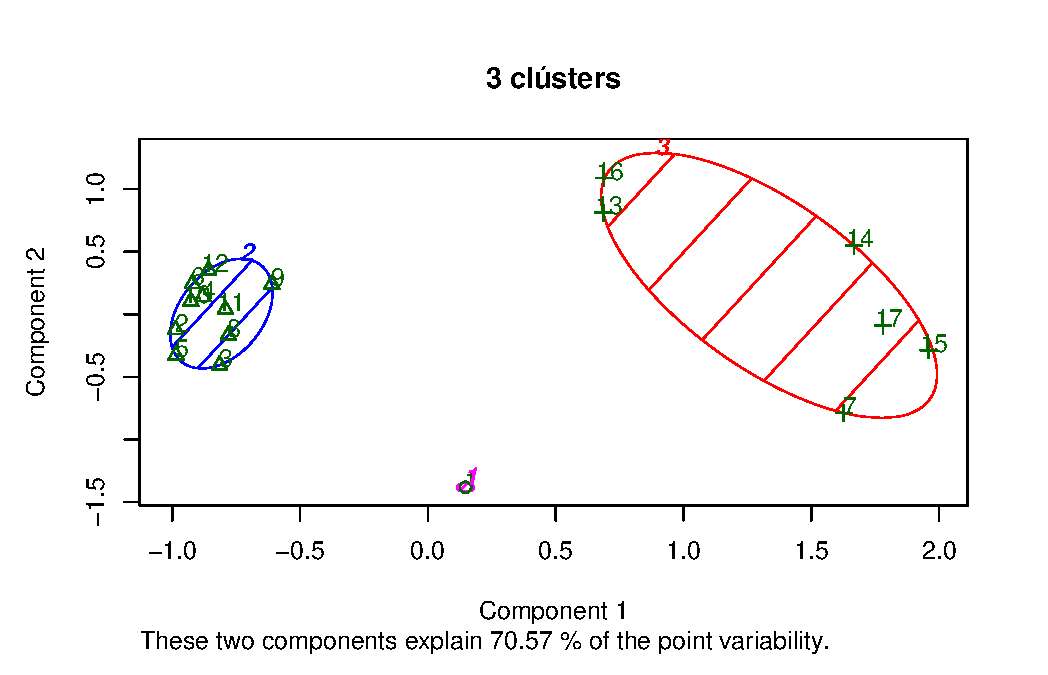
\includegraphics[scale=0.5]{clust3.eps}
\caption{\centering clusters resultantes con objetivo final 3. \\ \textbf{Fuente:} Elaboración propia haciendo uso de los datos de INE.}
\label{clust3}
\end{figure}

\begin{figure}[H]
\centering
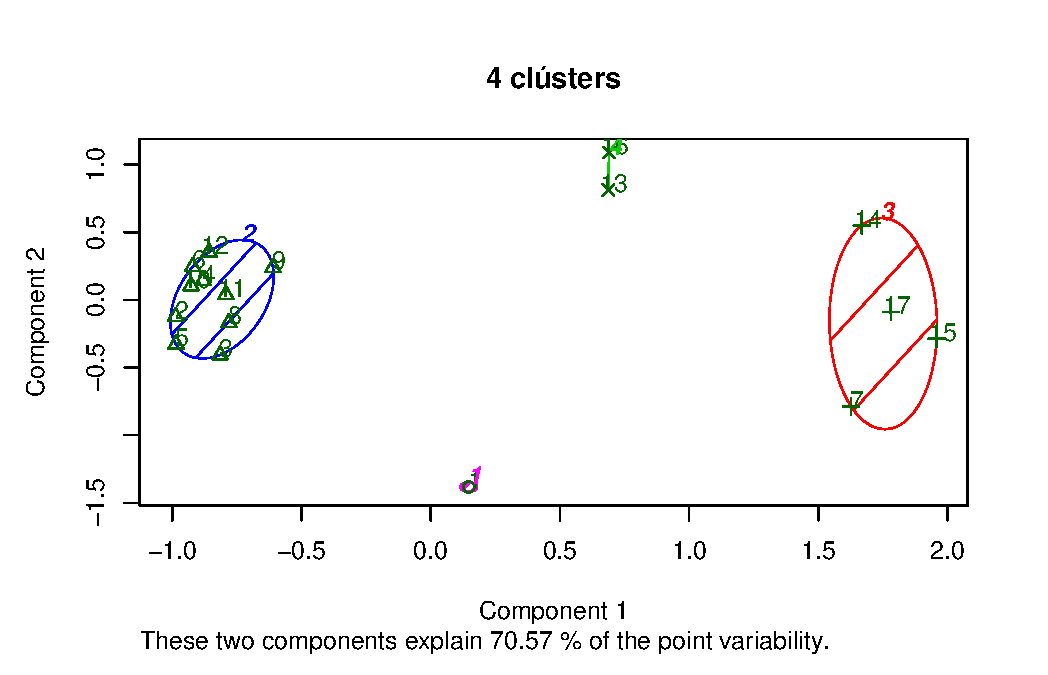
\includegraphics[scale=0.5]{clust4.eps}
\caption{\centering clusters resultantes con objetivo final 4. \\ \textbf{Fuente:} Elaboración propia haciendo uso de los datos de INE.}
\label{clust4}
\end{figure}

\begin{figure}[H]
\centering
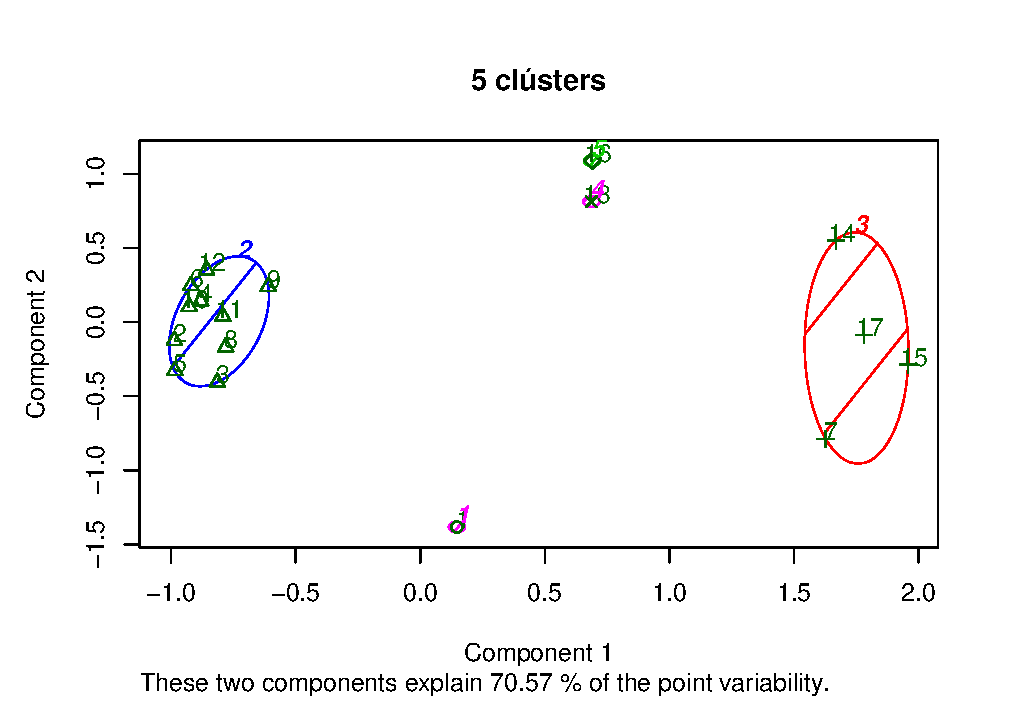
\includegraphics[scale=0.5]{clust5.eps}
\caption{\centering clusters resultantes con objetivo final 5. \\ \textbf{Fuente:} Elaboración propia haciendo uso de los datos de INE.}
\label{clust5}
\end{figure}



A partir de una representación por componentes principales que explican el 70.57\% de la variabilidad en las figuras \ref{clust3}, \ref{clust4} y \ref{clust5}, se pone de manifiesto la intuición que proporcionan las figuras  \ref{mapacalor} y \ref{em}, de manera que se evicencia que la elección quedará entre 3 o 4 clusters, aunque no es algo trivial y, como sucede en este caso, puede depender del punto de vista del analista. En esta ocasión, el número de clusters seleccionados es 4. En parte, esto viene respaldado en que los elementos de cada cluster han de ser lo más parecidos entre sí, pero que estas agrupaciones sean más homogéneas y simplifiquen el análisis, siempre evitando el exceso de ``singletons'', que son clusters con un solo elemento, y que se producirían en el caso de aumentar en más de 4 los clusters finales.

Para confirmar esta elección, se ha obtenido la silueta media de las agrupaciones de 3 y 4 clusters, para tomar un indicador cuantitativo objetivo. Los resultados son claros:


\begin{table}[H]
\centering
\begin{tabular}{|c|cc|}
\hline
\textbf{Silueta media} & 3 grupos  & 4 grupos  \\ \hline
cluster 1              & 0         & 0         \\
cluster 2              & 0.8478620 & 0.8416253 \\
cluster 3              & 0.4478921 & 0.5642511 \\
cluster 4              & -         & 0.6133732 \\ \hline
\end{tabular}
\caption{Siluetas medias para 3 y 4 clusters finales. \\ \textbf{Fuente:} Elaboración propia.}
\label{siluetas}
\end{table}


En el cuadro \ref{siluetas} se observa como seleccionar 4 clusters queda justificado ya que, si recordamos, la silueta marca la pertenencia a un conjunto de los elementos del mismo cluster, por lo que a mayor silueta, más seguridad se tendrá que los elementos de un cluster deben de pertenecer a éste, y como se puede observar, el escoger 4 clusters frente a 3 produce un notable aumento de las siluetas medias, a parte de que, siguiendo el razonamiento de \cite{fgd}, es menos óptima una agrupación con una estructura fuerte y una débil  (que presenta la agrupación con 3 clusters finales) a una estructura fuerte y dos estructuras razonables (que aparece con 4 grupos finales) (Apartado 3.5).

\vspace{0.3cm}

Otro algoritmo diferente que permite visualizar las posibles agrupaciones son las técnicas de clustering jerárquico, ya que no requieren de un número de grupos finales desde un inicio, sino que bajo la previa definición de una distancia se podrán dibujar directamente los dendrogramas correspondientes. La distancia que se utilizará es 1-correlación, la cual cumple trivialmente los tres axiomas de disimilaridad. Realizándolo para tres métodos distintos, el single, el complete y el ward, se obtienen resultados que concuerdan con lo observado anteriormente.


\begin{figure}[H]
\centering
\includegraphics[scale=0.5]{dendrsingle.eps}
\caption{\centering Dendrograma con el método single. \\ \textbf{Fuente:} Elaboración propia.}
\label{dendr1}
\end{figure}

\begin{figure}[H]
\centering
\includegraphics[scale=0.5]{dendrcomplete.eps}
\caption{\centering Dendrograma con el método complete. \\ \textbf{Fuente:} Elaboración propia.}
\label{dendr2}
\end{figure}

\begin{figure}[H]
\centering
\includegraphics[scale=0.5]{dendrward.eps}
\caption{\centering Dendrograma con el método ward. \\ \textbf{Fuente:} Elaboración propia.}
\label{dendr3}
\end{figure}


Queda justificado en las figuras \ref{dendr1}, \ref{dendr2} y \ref{dendr3},  que los resultados que se obtienen con PAM son consistentes, ya que los tres métodos representan resultados muy parecidos para los distintos métodos utilizados. Se decide así crear 4 agrupaciones de causas de mortalidad entre las que los elementos que pertenecen al mismo grupo habrán evolucionado históricamente de una manera similar.

\vspace{0.3cm}

En el cuadro \ref{nomclust} se puede observar cuáles son las causas que se han agrupado, con el nombre de cada causa y el cluster al que corresponden.

\begin{table}[H]
\centering
\begin{tabular}{ccc}
Cluster & Causa        & Nombre completo    \\ \hline \hline
1     &  1  & 001-008  I.Enfermedades infecciosas y parasitarias (1)                              \\ \hline
2                            & 2  & 009-041  II.Tumores                                                                 \\
2                            & 3  & 042-043  III.Enfermedades de la sangre y de los órganos hematopoyéticos,            \\
                           &                 & y ciertos trastornos que afectan al mecanismo de la inmunidad                       \\
2                            & 4  & 044-045  IV.Enfermedades endocrinas, nutricionales y metabólicas                    \\
2                            & 5  & 046-049  V.Trastornos mentales y del comportamiento                                 \\
2                            & 6  & 050-052  VI-VIII.Enfermedades del sistema nervioso y de los órganos de los sentidos \\
2                            & 8  & 062-067  X.Enfermedades del sistema respiratorio                                    \\
2                            & 9  & 068-072  XI.Enfermedades del sistema digestivo                                      \\
2                            & 10 & 073  XII.Enfermedades de la piel y del tejido subcutáneo                            \\
2                            & 11 & 074-076  XIII.Enfermedades del sistema osteomuscular y del tejido conjuntivo        \\
2                            & 12 & 077-080  XIV.Enfermedades del sistema genitourinario                                \\ \hline
3                            & 7  & 053-061 IX.Enfermedades del sistema circulatorio                                    \\
3                            & 14 & 082  XVI.Afecciones originadas en el periodo perinatal                              \\
3                            & 15 & 083-085  XVII.Malformaciones congénitas, deformidades y anomalías cromosómicas      \\
3                            & 17 & 090-102,XX.Causas externas de mortalidad                                            \\ \hline
4                            & 13 & 081,XV.Embarazo, parto y puerperio                                                  \\
4                            & 16 & 086-089,XVIII.Síntomas, signos y hallazgos anormales clínicos y de laboratorio,     \\
                             &                 & no clasificados en otra parte (2)                                                  
\end{tabularx}
\caption{Agrupación de las causas por clusters. \\ \textbf{Fuente:} Elaboración propia.}
\label{nomclust}
\end{table}

Se pasará ahora a estudiar cada uno de los grupos creados por separado, empezando por la evolución que presentan a lo largo de todos los años estudiados (1987-2014).

\subsection{Estudio de los clusters}

La agrupación de cauasa de mortalidad según la clusterización la utilizaremos para poder predecir cómo va a ser la mortalidad en esas agrupaciones por separado. Inicialmente, se mostrará en la figura \ref{distrclust} muestra el número de fallecidos total en 2014 para cada una de las agrupaciones realizadas. Se observa en la figura \ref{distrclust}, y es consistente con la realización de las agrupaciones, que los clusters 1 y 4 incluyen muy pocas defunciones en comparación con los clusters 2 y 3. Esto indica que la tendencia de la mortalidad total dependerá en mayor medida de estos dos grandes clusters, es decir, si se analizara la evolución conjunta de la mortalidad, dominaría la tendencia que marcan los grupos con un mayor número de fallecidos. Aún así, se propone modelizar los cuatro clusters a partir de los modelos de Lee-Carter ya estudiados. 

\begin{figure}[H]
\centering
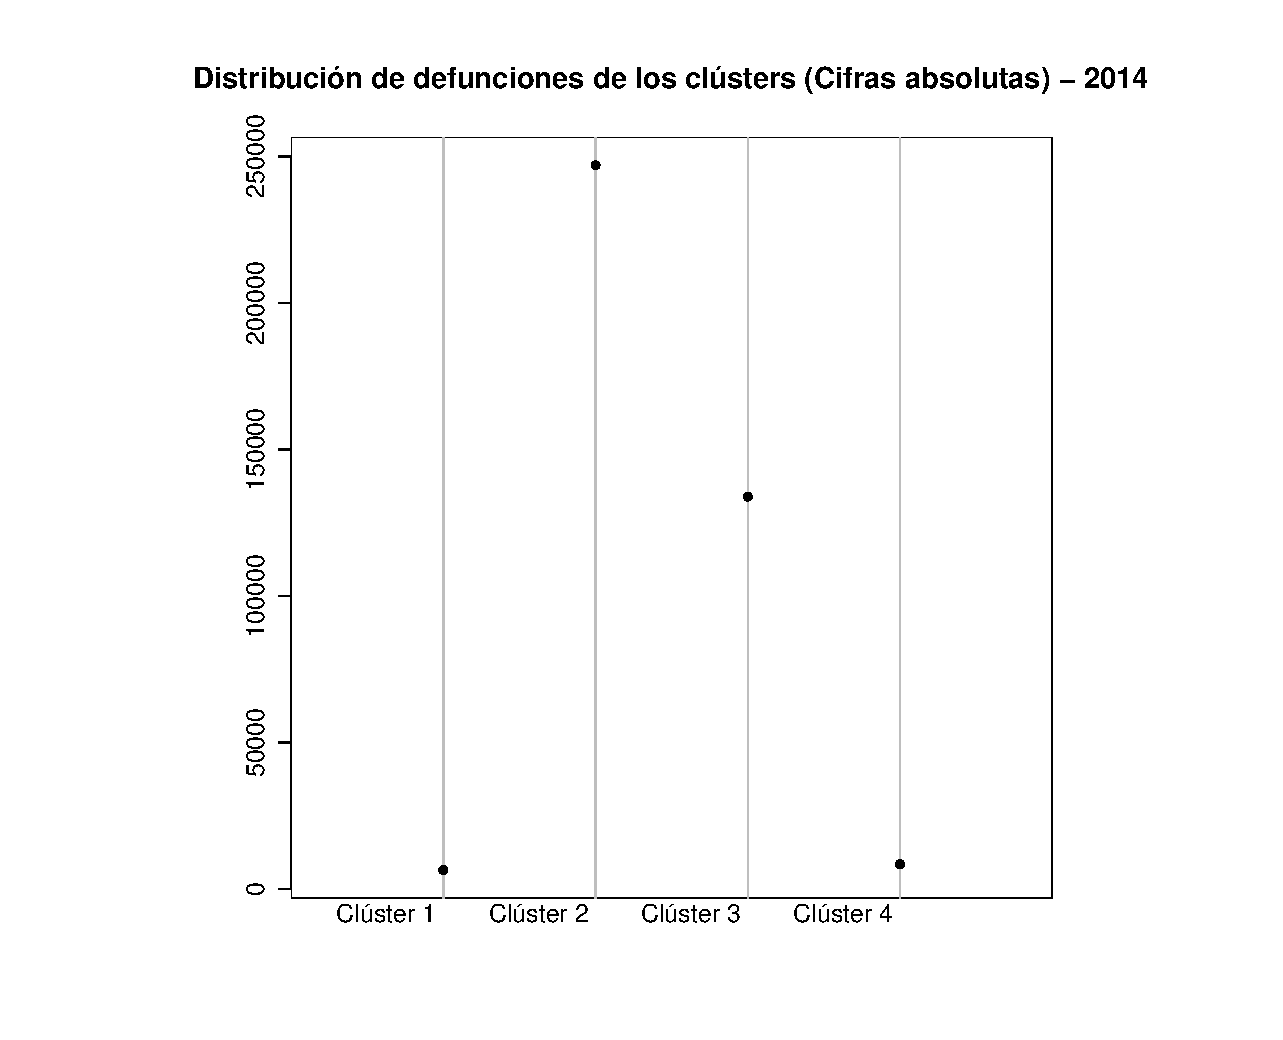
\includegraphics[scale=0.3]{distrclust.eps}
\caption{\centering Distribución de la mortalidad en cada cluster. \\ \textbf{Fuente:} Elaboración propia.}
\label{distrclust}
\end{figure}

\begin{figure}[H]
\centering
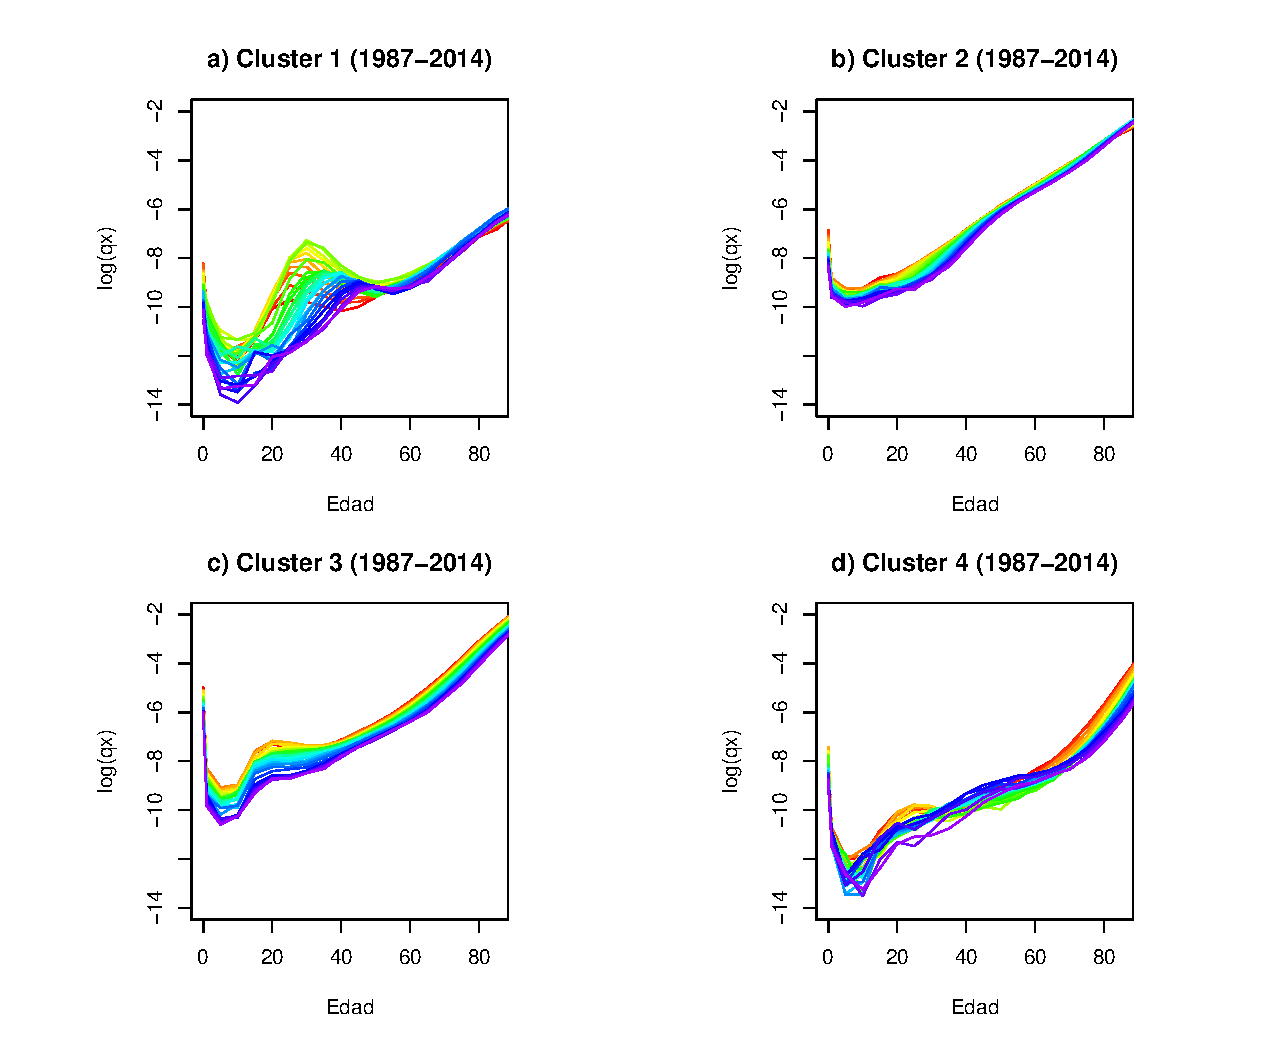
\includegraphics[scale=0.65]{clustevofunction.eps}
\caption{\centering Evolución de la mortalidad en cada cluster por año. \\ \textbf{Fuente:} Elaboración propia.}
\label{clustevol}
\end{figure}

Se aprecia en la figura \ref{clustevol} como el cluster 1, formado sólo por la causa 1 (Enfermedades infecciosas y parasitarias), presenta una joroba con una varianza muy alta a lo largo de estos últimos 27 años. Se observa como la mortalidad entre las edades 20 y 40 ha ido creciendo durante varios años y se ha mantenido elevada desde entonces, siendo actualmente, la tasa en 2014 a los 40 años superior a la del 1987. Esto provoca un desplazamiento de la joroba de accidentes que situaba su pico a los 25 años en 1987 y en 2014 lo sitúa en los 40 años. 

\vspace{0.3cm}
Se observa por otra parte que en el cluster 2 no se presenta una gran variación de la mortalidad a lo largo de los años, pese al gran volumen de fallecimientos que engloba. Se aprecia una disminución continuada de la mortalidad, aunque la joroba social que se produce entorno a los 25 años para las enfermedades del cluster 1 en este caso no sólo no se produce, sino que parece que sea en sentido inverso, mientras que recupera su ``tendencia natural'' a los 50 años.

\vspace{0.3cm}
El tercer cluster presenta la forma característica del modelo de Helligman-Pollard, de manera que se aprecian tres partes claramente diferenciadas: Adaptación, de 0 a 1 años, joroba social, de 1 a 35 años, y longevidad natural, que engloba edades superiores a 35 años.

\vspace{0.3cm}
El cuarto y último cluster tiene unas tasas muy reducidas al igual que el primero, lo cual es debido principalmente a las pocas causas que engloban, aunque presenta una varianza notable, lo que indica la gran variación que han tenido las defunciones por estas causas. Se puede observar como en estos últimos 5 años la mortalidad entre los 40 y 60 años ha ido en aumento y se mantiene por encima de años anteriores en los que presentaba un descenso claro. Recordar que las causas que forman este cluster son \emph{embarazo, parto y puerperio} y \emph{síntomas, signos y hallazgos anormales clínicos y de laboratorio}. 

\vspace{0.3cm}

La evolución de la mortalidad en cada cluster puede visualizarse desde otra perspectiva en la figura \ref{clustevol}, que representan la evolución de todos los grupos de edad a lo largo de los años frente a las tasas de mortalidad de cada uno de los clusters. 

\begin{figure}[H]
\centering
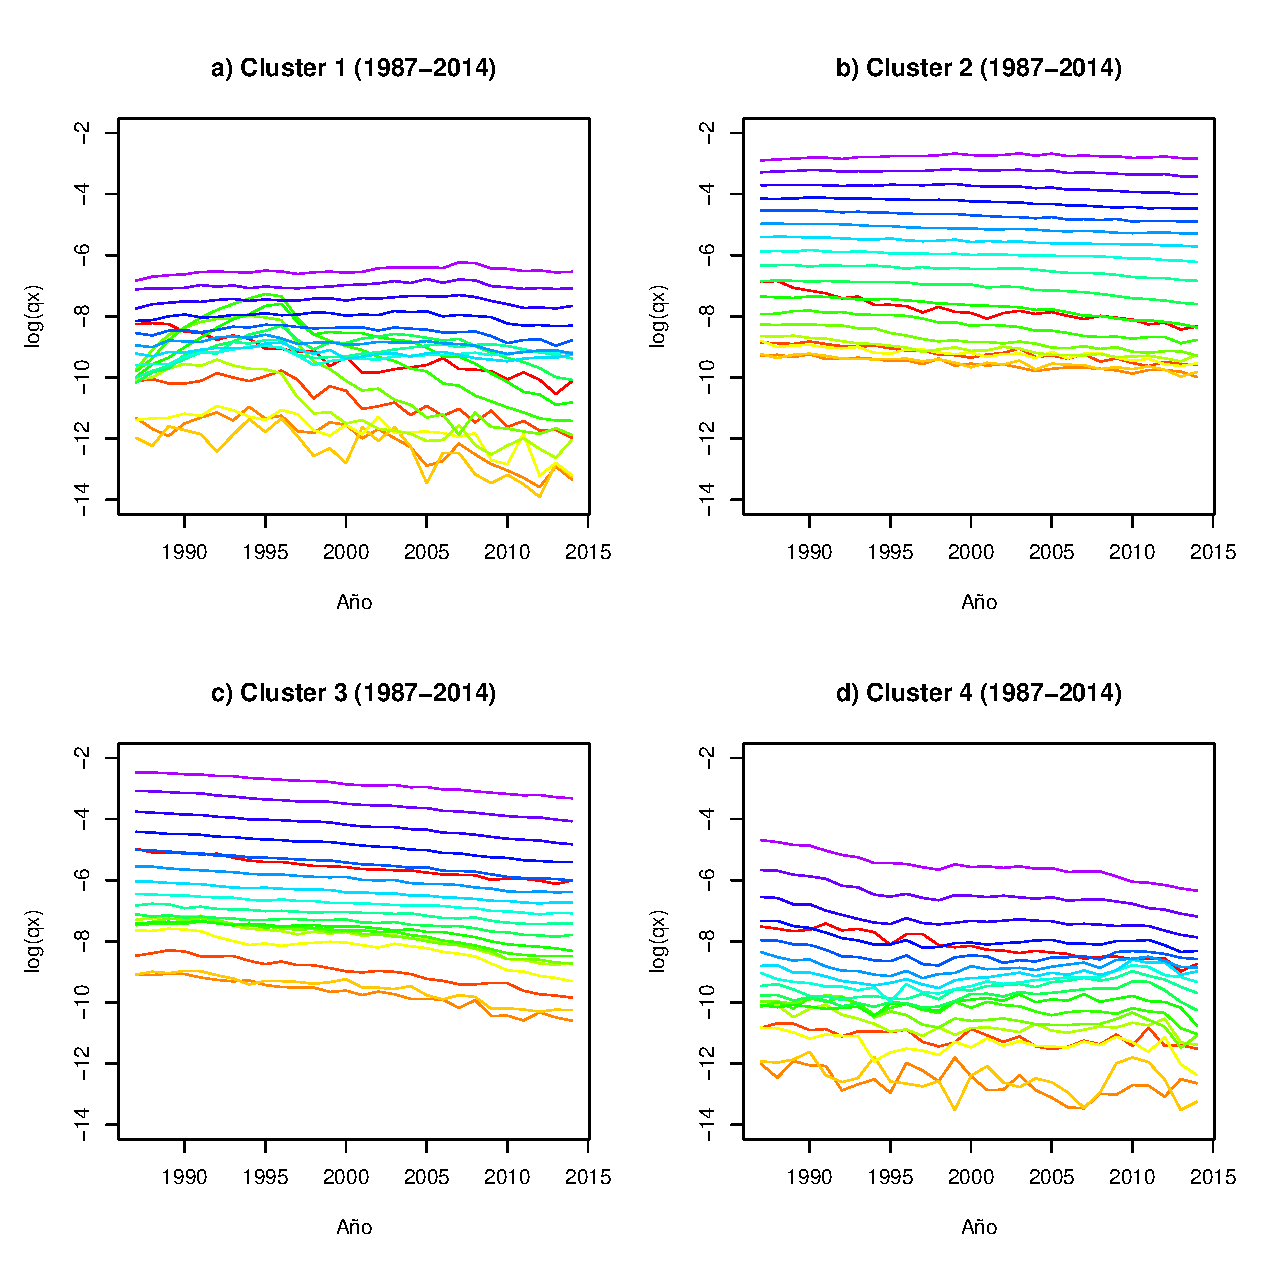
\includegraphics[scale=0.6]{clustevotime.eps}
\caption{\centering Evolución de la mortalidad en cada cluster por grupos de edad. \\ \textbf{Fuente:} Elaboración propia.}
\label{clustevotime}
\end{figure}

En la figura  \ref{clustevotime} se observa la diferencia de evolución de la mortalidad en cada cluster por grupos de edad. Como ya se sabe, los grupos de edad pueden ser agrupados en tres grandes grupos, la adaptación al medio, que en este gráfico queda representada por los colores más cálidos, la joroba social, que está representado por los más verdosos, y la longevidad natural, representada con los colores más fríos. Se observa principalmente como en todos los clusters, la adaptación al medio es más crítica que una gran cantidad, lo que en la curva de mortalidad es la bajada que aparece en las edades más bajas, lo que aquí viene representado con la línea roja cerca de colores que no se asemejan. Cabe notar que una mortalidad lineal produciría una distribución similar a la de un arcoiris en este gráfico.

La variabilidad que se comentaba sobre los clusters 1 y 4 se puede observar más claramente en las figuras 15a y 15d, al visualizar cómo las lineas no son rectas, sino que presentan distintos picos. Esto indica que las causas incluidas en estos clusters no han evolucionado de una manera similar para los distintos grupos de edad, siendo los más jóvenes los que han presentado más variación y las edades más altas las que han evolucionado más establemente.

Otro aspecto a destacar es el significado de la separación entre las líneas, que nos indica cuál es la pendiente que presentará la curva de mortalidad, es decir, cuanto más separadas estén las lineas correspondientes a dos grupos de edad, más será la diferencia de las tasas de mortalidad al pasar de un grupo de edad a otro. Esto se puede observar en los clusters 3 y 4 en las edades más tempranas, en las que se ve que para pasar de los grupos de edades correspondientes a los colores amarillo, de 10 a 14 años, y naranja, de 15 a 19 años, se produce un aumento muy notable de la mortalidad. Al contrario ocurre en las edades de 25 a 40 años, pintadas con distintas tonalidades de verde, donde la pequeña separación que tienen sus lineas de evolución en el tiempo indica que la curva de tasas de mortalidad presentará una subida muy poco acentuada durante el paso entre estas edades.

Se pasará ahora a ajustar con los modelos de Lee-Cartes ya explicados cada uno de los clusters. También se ajustará la mortalidad total sin desagregar para comparar las predicciones.

\subsection{Modelo de Lee-Carter: Ajuste y predicción por cluster}

En esta sección se exponen los resultados correspondientes a los ajustes a partir de los modelos de Lee-Cartes para cada una de las agrupaciones. Inicialmente expondremos e interpretaremos los parámetros resultantes para cada uno de los clusters como para el modelo sin desagregar por causas de mortalidad, con el objetivo de poder observar las mejoras obtenidas. Seguidamente presentaremos la predicción de la mortalidad total por ambos modelos, el total sin desagregar por causas y el obtenido por agregar los resultados de los 4 modelos correspondientes a cada uno de los clusters. Finalmente presentaremos la predicción a largo plazo para poder comparar la estabilidad de ambos modelos, concluyendo que la desagregación produce una mayor estabilidad y consistencia en la predicción.

Se han realizado los modelos correspondientes de Lee-Carter para cada uno de los clusters y para el total sin desagregar, con el propósito de poder comparar ambas predicciones. Recordar que el modelo de Lee-Carter,  como se ha mencionado en la metodología, tenía 3 parámetros principales, dos relacionados con la edad ($a_{x}$ y $b_{x}$) y uno con el tiempo ($k_{t}$), y predice el tanto central de mortalidad a partir de la ecuación \ref{leecarter}. Los parámetros que se obtienen para todos los modelos son los que siguen\footnote{Las tablas completas se pueden encontrar en \url{https://github.com/JuanJoseVidal/Mortalidad-por-causas.-Desagregaci-n-y-predicci-n./tree/master/Tablas}.}:

\begin{table}[H]
\centering
\begin{tabular}{c|cc|cc|cc|cc|cc}
             & \multicolumn{2}{c}{Total} & \multicolumn{2}{c}{Cluster 1} & \multicolumn{2}{c}{Cluster 2} & \multicolumn{2}{c}{Cluster 3} & \multicolumn{2}{c}{Cluster 4} \\ \hline
\textbf{Edad} & $a_x$       & $b_x$       & $a_x$          & $b_x$        & $a_x$         & $b_x$         & $a_x$         & $b_x$         & $a_x$          & $b_x$        \\ \hline
0            & -5.78       & -0.00       & -9.32          & 0.01         & -8.49         & -0.02         & -5.59         & 0.01          & -8.32          & 1.04         \\
1            & -7.71       & 0.02        & -10.78         & 0.02         & -9.29         & 0.00          & -8.77         & 0.01          & -10.97         & -0.27        \\
2            & -8.08       & 0.03        & -11.27         & 0.02         & -9.45         & 0.01          & -9.33         & 0.01          & -11.56         & -0.54        \\
3            & -8.26       & 0.03        & -11.59         & 0.02         & -9.52         & 0.01          & -9.56         & 0.01          & -11.86         & -0.67        \\
4            & -8.35       & 0.03        & -11.82         & 0.02         & -9.55         & 0.01          & -9.63         & 0.01          & -12.03         & -0.72        \\
5            & -8.39       & 0.03        & -11.98         & 0.02         & -9.56         & 0.01          & -9.63         & 0.01          & -12.11         & -0.74        \\
6            & -8.39       & 0.03        & -12.08         & 0.02         & -9.56         & 0.01          & -9.57         & 0.01          & -12.13         & -0.72        \\
7            & -8.37       & 0.02        & -12.13         & 0.02         & -9.55         & 0.01          & -9.47         & 0.01          & -12.10         & -0.69        \\
8            & -8.33       & 0.02        & -12.15         & 0.02         & -9.52         & 0.01          & -9.35         & 0.01          & -12.05         & -0.64        \\
9            & -8.29       & 0.02        & -12.14         & 0.02         & -9.49         & 0.01          & -9.21         & 0.01          & -11.97         & -0.58        \\
10           & -8.23       & 0.02        & -12.10         & 0.02         & -9.46         & 0.01          & -9.07         & 0.01          & -11.87         & -0.51   \\
   \vdots          & \vdots       & \vdots        & \vdots        & \vdots         & \vdots         & \vdots          & \vdots         & \vdots          & \vdots        & \vdots 
\end{tabular}
\caption{Parámetros $a_{x}$ y $b_{x}$ de los distintos modelos\\ \textbf{Fuente:} Elaboración propia.}
\end{table}


\begin{table}[H]
\centering
\begin{tabular}{c|c|cccc}
 \textbf{Año} & $k_{t}$ Total & $k_{t}$ Clust. 1  & $k_{t}$ Clust. 2 & $k_{t}$ Clust. 3 & $k_{t}$ Clust. 4 \\ 
  \hline
1987 & 41.09 & -29.38 & 14.95 & 45.13 & 1.68 \\ 
  1988 & 41.88 & -47.34 & 18.50 & 44.77 & 1.63 \\ 
  1989 & 40.71 & 4.98 & 19.95 & 42.56 & 1.31 \\ 
  1990 & 41.65 & 24.36 & 26.38 & 40.63 & 1.36 \\ 
  1991 & 39.49 & 36.79 & 23.50 & 38.99 & 1.00 \\ 
  1992 & 33.30 & 45.65 & 18.93 & 32.36 & 0.60 \\ 
  1993 & 34.40 & 53.63 & 22.76 & 31.39 & 0.52 \\ 
  1994 & 29.52 & 56.43 & 22.01 & 25.01 & 0.05 \\ 
  1995 & 28.55 & 61.58 & 23.19 & 22.00 & 0.01 \\ 
\vdots&\vdots&\vdots&\vdots&\vdots&\vdots
\end{tabular}
\caption{Parámetros $k_{t}$ de los distintos modelos\\ \textbf{Fuente:} Elaboración propia.}
\end{table}



Para poder observar de dónde se obtiene cada una de las tendencias, se representan los distintos factores obtenidos para así poder compararlos:


\begin{figure}[H]
\centering
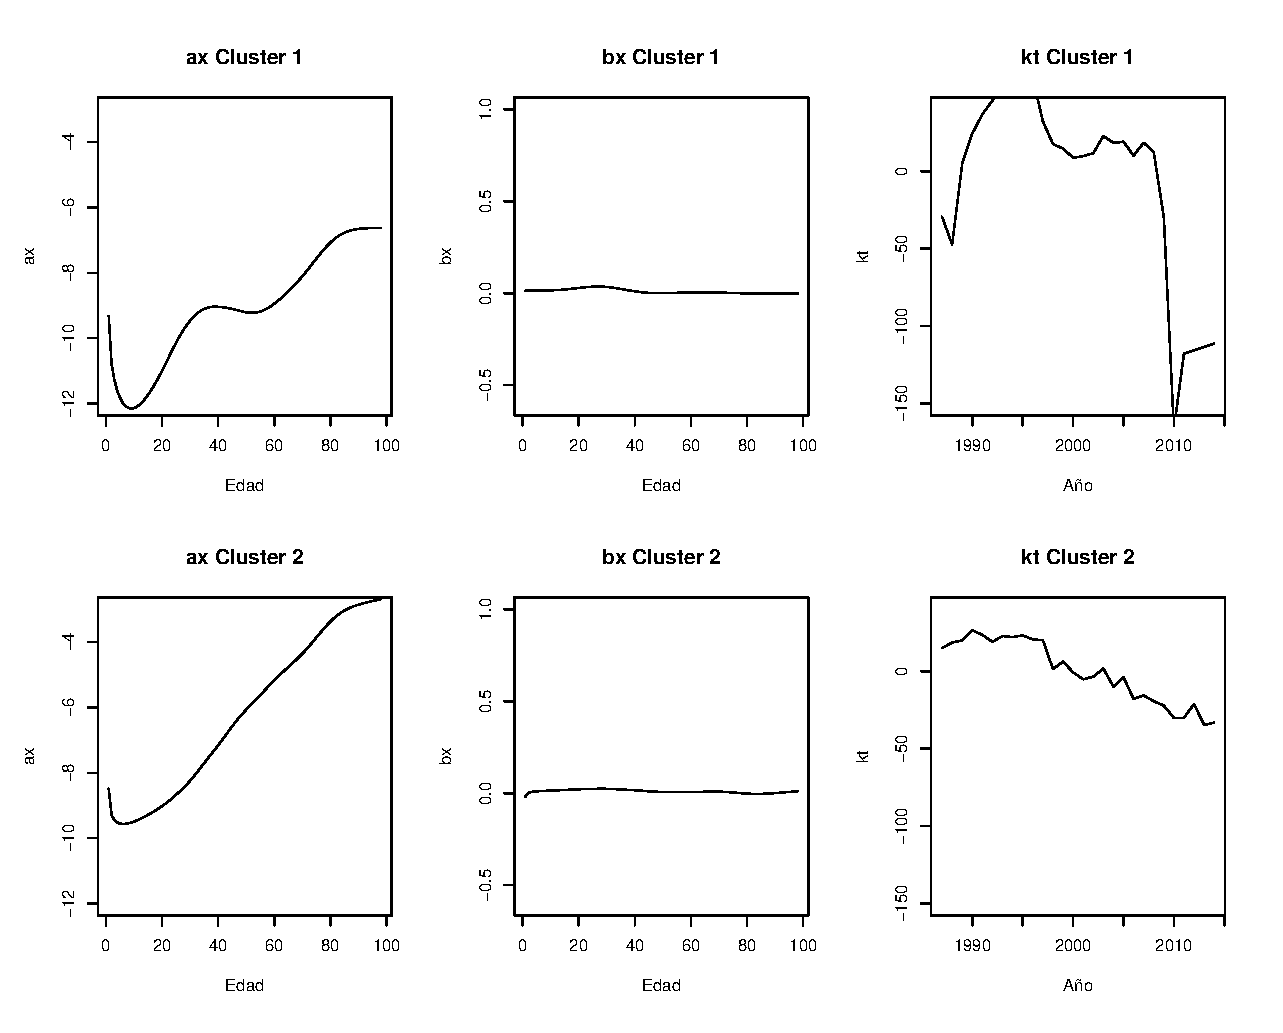
\includegraphics[scale=0.45]{pars12.eps}
\caption{\centering Parámetros $a_{x}$, $b_{x}$ y $k_{t}$ de los modelos de Lee-Carter obtenidos para los clusters 1 y 2. \\ \textbf{Fuente:} Elaboración propia.}
\label{params12}
\end{figure}

\begin{figure}[H]
\centering
\includegraphics[scale=0.45]{pars34.eps}
\caption{\centering Parámetros $a_{x}$, $b_{x}$ y $k_{t}$ de los modelos de Lee-Carter obtenidos para los clusters 3 y 4. \\ \textbf{Fuente:} Elaboración propia.}
\label{params34}
\end{figure}

Para analizar los efectos de la mortalidad exclusivos para cada una de las edades, podemos utilizar el coeficiente $a_{x}$ que nos proporciona el ajuste de Lee-Carter.
Se aprecia como en los gráficos de la izquierda en las figuras \ref{params12} y \ref{params34} se encuentran las $a_{x}$, que representan los efectos de la mortalidad exclusivos de las edades. Se observa como estas curvas representan una suavización de la curva de mortalidad en escala logarítmica, que se verá afectada por los otros factores siguiendo la ecuación \ref{leecarter}.

\vspace{0.3cm}

En la columna central de las figuras \ref{params12} y \ref{params34} aparecen las distintas $b_{x}$ del modelo de Lee-Carter, que representan las constantes respecto a la edad indicando qué tasas decrecen más lentamente en respuesta a los cambios y la variación del tiempo, la única en la que las $b_{x}$ afectan significativamente al modelo es en el cluster 4. 

\vspace{0.3cm}

Al contrario que lo que ocurre con las $b_{x}$ ocurre con las $k_{t}$, que muestran cierta variación anómala para el cluster 1 y un acentuado decrecimiento para los clusters 2 y 3. Lo que indican principalmente estos gráficos es que la tendencia para los tres primeros clústers depende de su evolución a lo largo de los años, mientras que para el cuarto depende fundamentalmente de la edad en la que se encuentre. Notar que a estos parámetros habría que introducir los residuales $\varepsilon_{x,t}$, que no han sido presentados, para obtener el modelo completo.

Si se toman los datos reales del INE de defunciones y supervivientes para el año 2015, se podrán validar los modelos y observar cómo se han predicho los datos para el año 2015:

\begin{figure}[H]
\centering
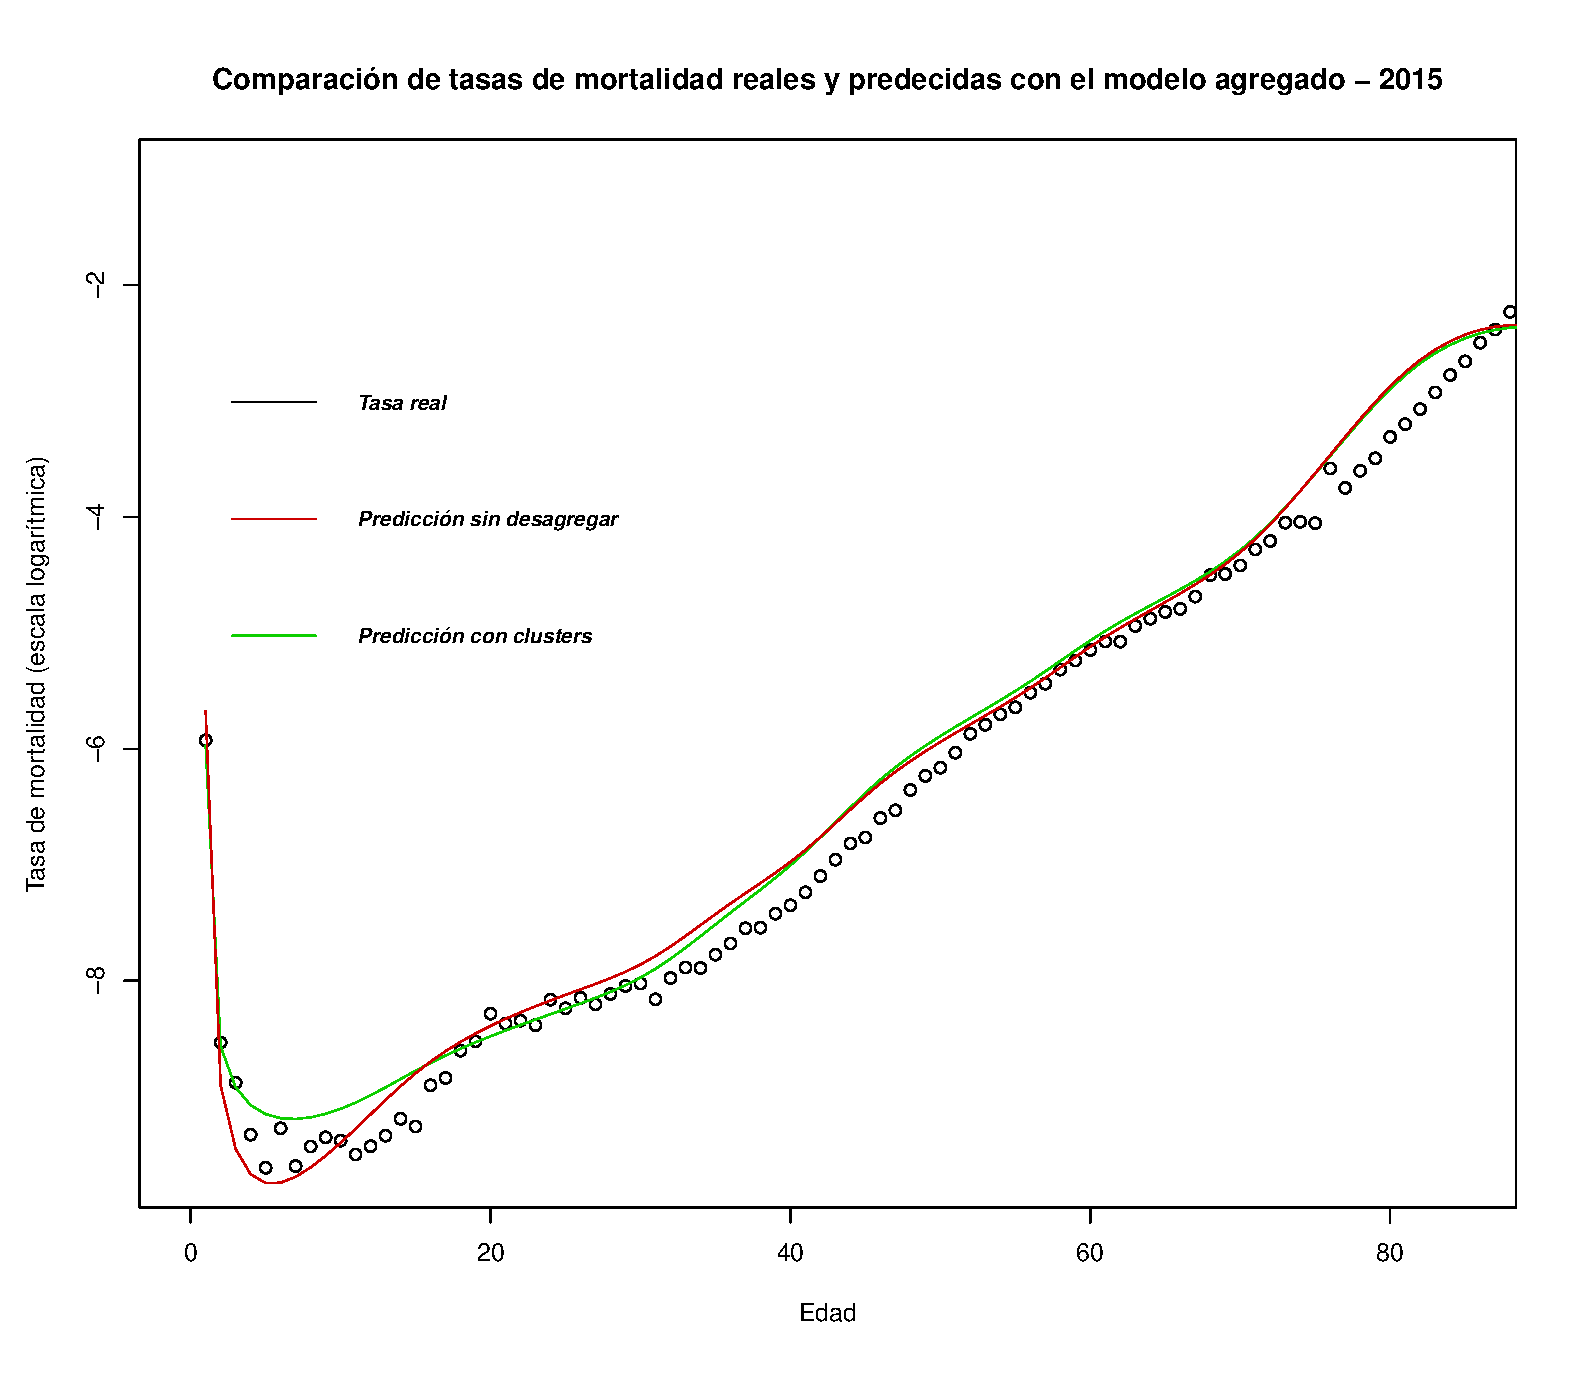
\includegraphics[scale=0.4]{predict2015.eps}
\caption{\centering Comparación de las predicciones de la mortalidad total para 2015. \\ \textbf{Fuente:} Elaboración propia.}
\label{prediction2015}
\end{figure}

En el que se observa cómo las predicciones han sido muy precisas, donde cabe destacar con qué precisión se ajusta la caída de adaptación al medio y en las edades más tempranas, llegando sólo a producirse un mínimo error entre las edades 10 y 20, en el cual se sobreestima la mortalidad esperada para estas edades. Notar también cómo la curva de accidentes de los años 35 a 45 años queda ligeramente más alta que la que realmente se ha observado. Para el modelo agregado se observa como se infraestima la mortalidad para las edades más tempranas y empieza a sobreestimar a partir de los 10 años para todo el rango de edades. 

La comparación de predicciones a un año no resulta del todo aclaratoria y es difícil elegir qué modelo es mejor, por lo que se ha decidido presentar cómo evolucionarían a largo plazo las predicciones. En la figura \ref{comparaciontotal} se comprueba como el modelo por agregaciones produce una mayor estabilidad muy valiosa en el caso de realizar predicciones a largo plazo.

Para poder realizar una mejor comparación de los modelos, se decide representar las predicciones de las $q_{x}$ para los futuros años. Es así como se observa que, al desagregar por clusters, si se suman las $q_{x}$ de todos los modelos de las agrupaciones se obtendrá una aproximación de la mortalidad total (ecuación \ref{equivcaus}), y si se compara con el modelo obtenido sin desagregar, se observa que las predicciones para una gran cantidad de edades no varía excepto entre los años 0 y 10, donde claramente se observa que la desagregación (\textcolor{green}{verde}) produce una mayor estabilidad en la predicción que sin desagregar (\textcolor{red}{rojo}), lo cual nos indica que el modelo obtenido a partir de las causas mejora el modelo obtenido sin desagregar por éstas.


\begin{figure}[H]
 \centering
  \subfloat{
    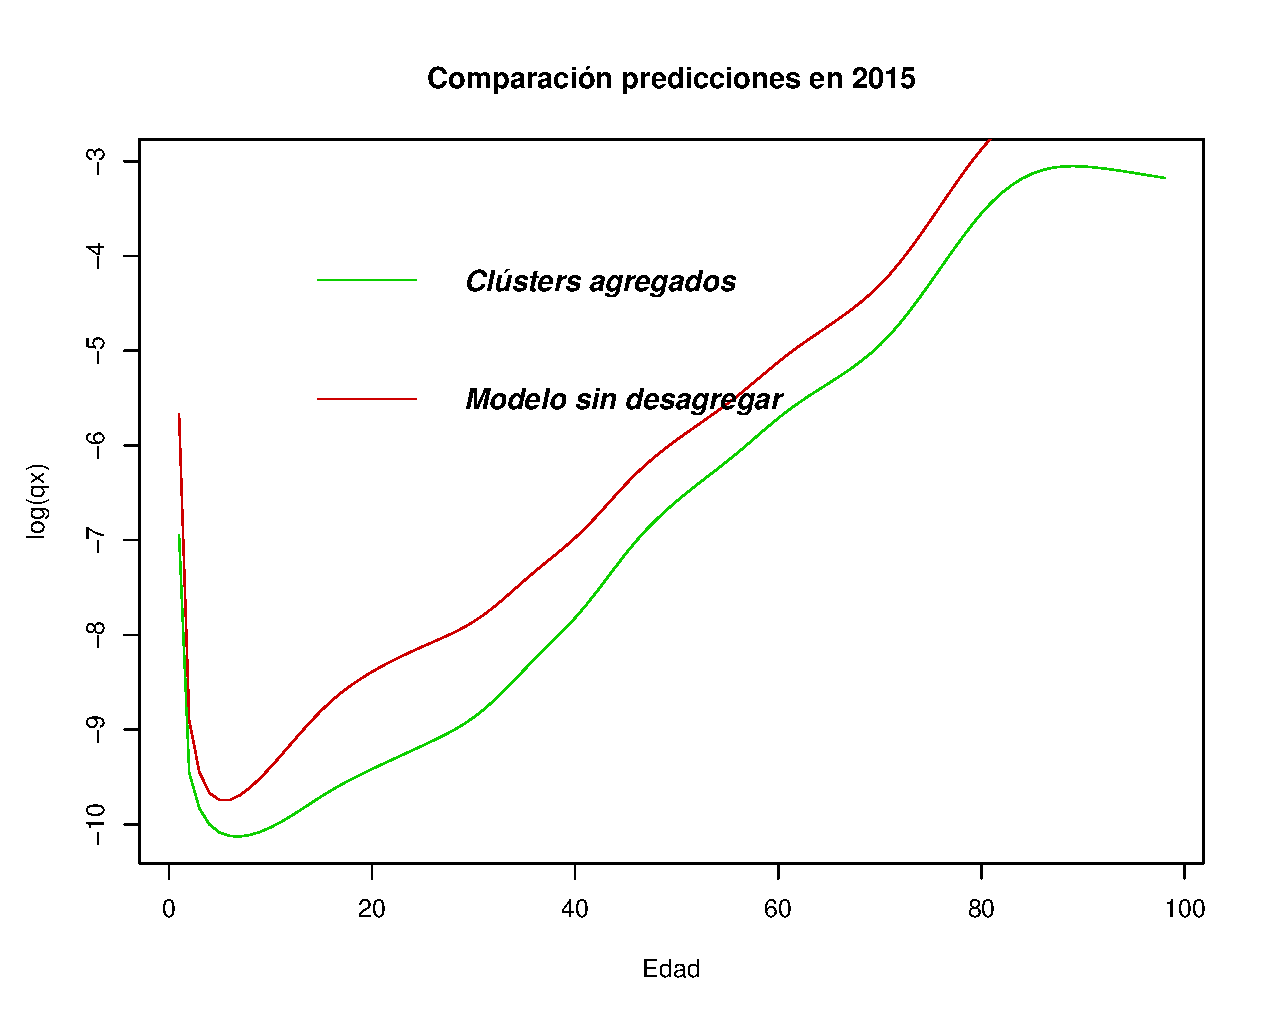
\includegraphics[width=0.55\textwidth]{comp15.eps}}
  \subfloat{
    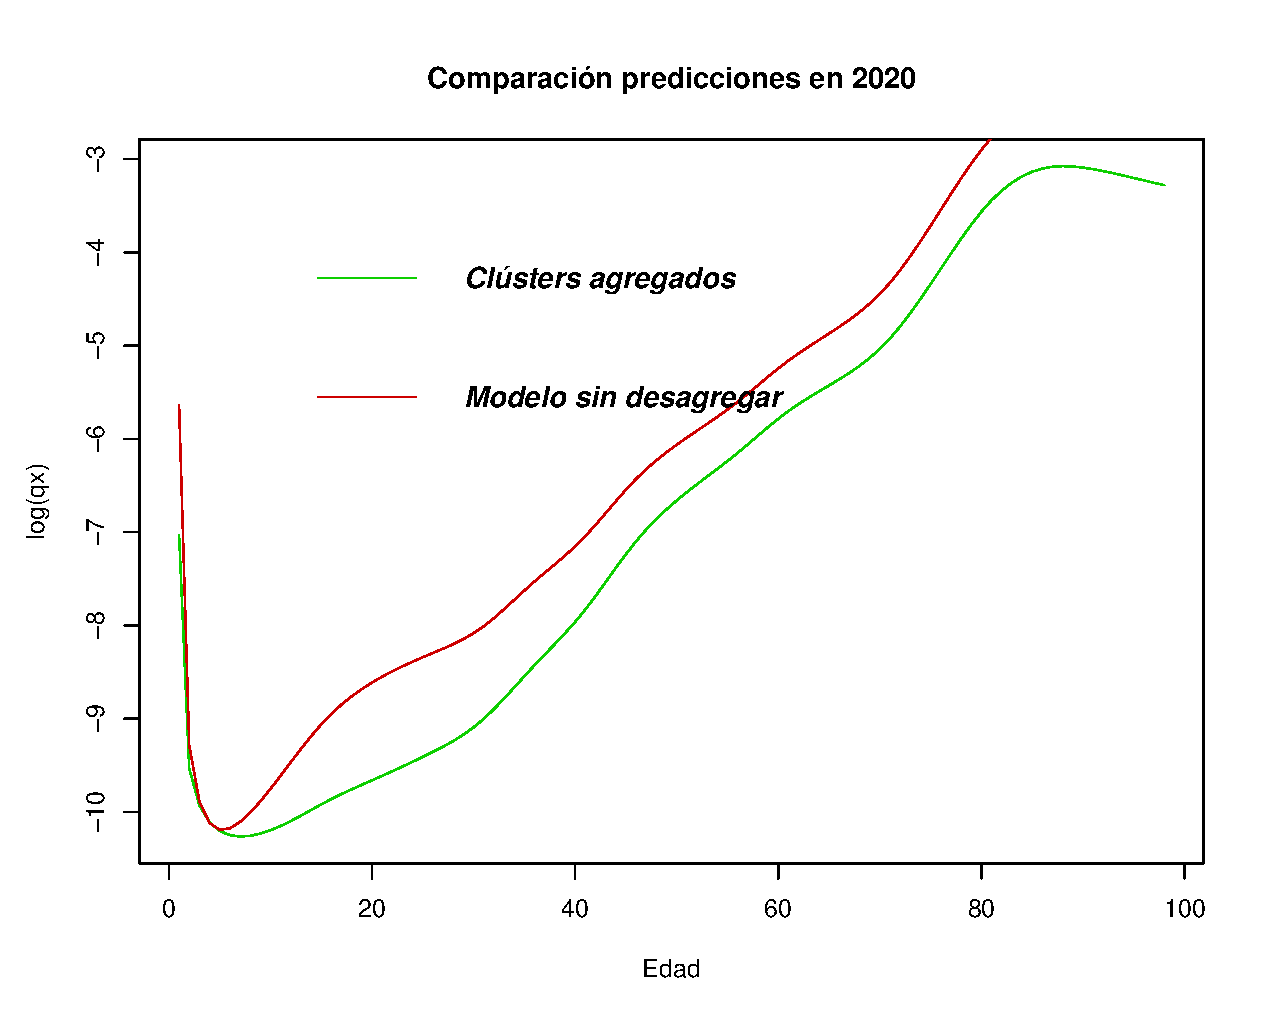
\includegraphics[width=0.55\textwidth]{comp20.eps}}
\end{figure}

\begin{figure}[H]
 \centering
  \subfloat{
    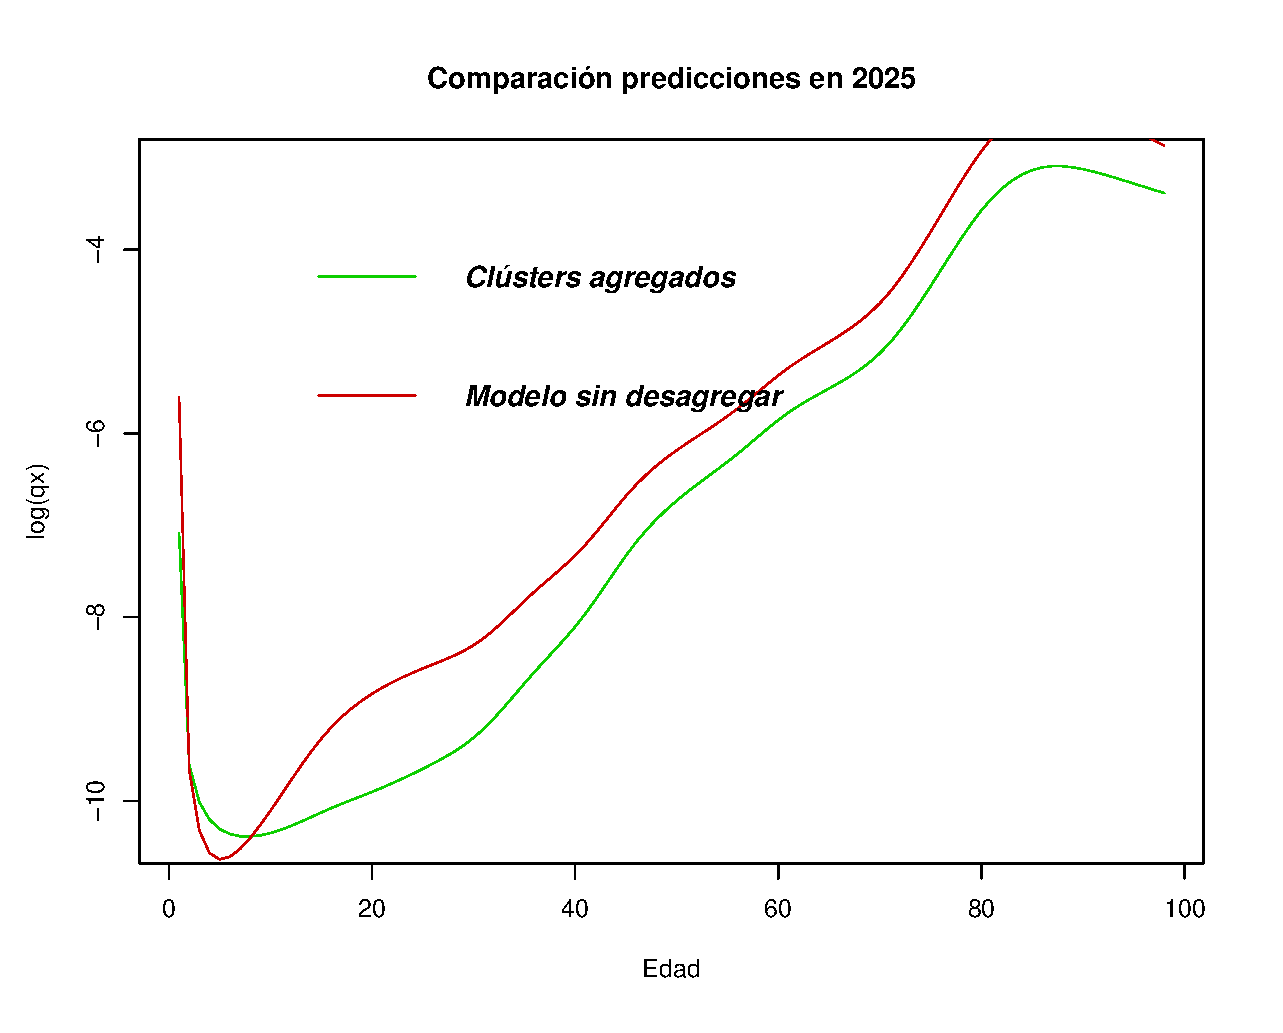
\includegraphics[width=0.55\textwidth]{comp25.eps}}
  \subfloat{
    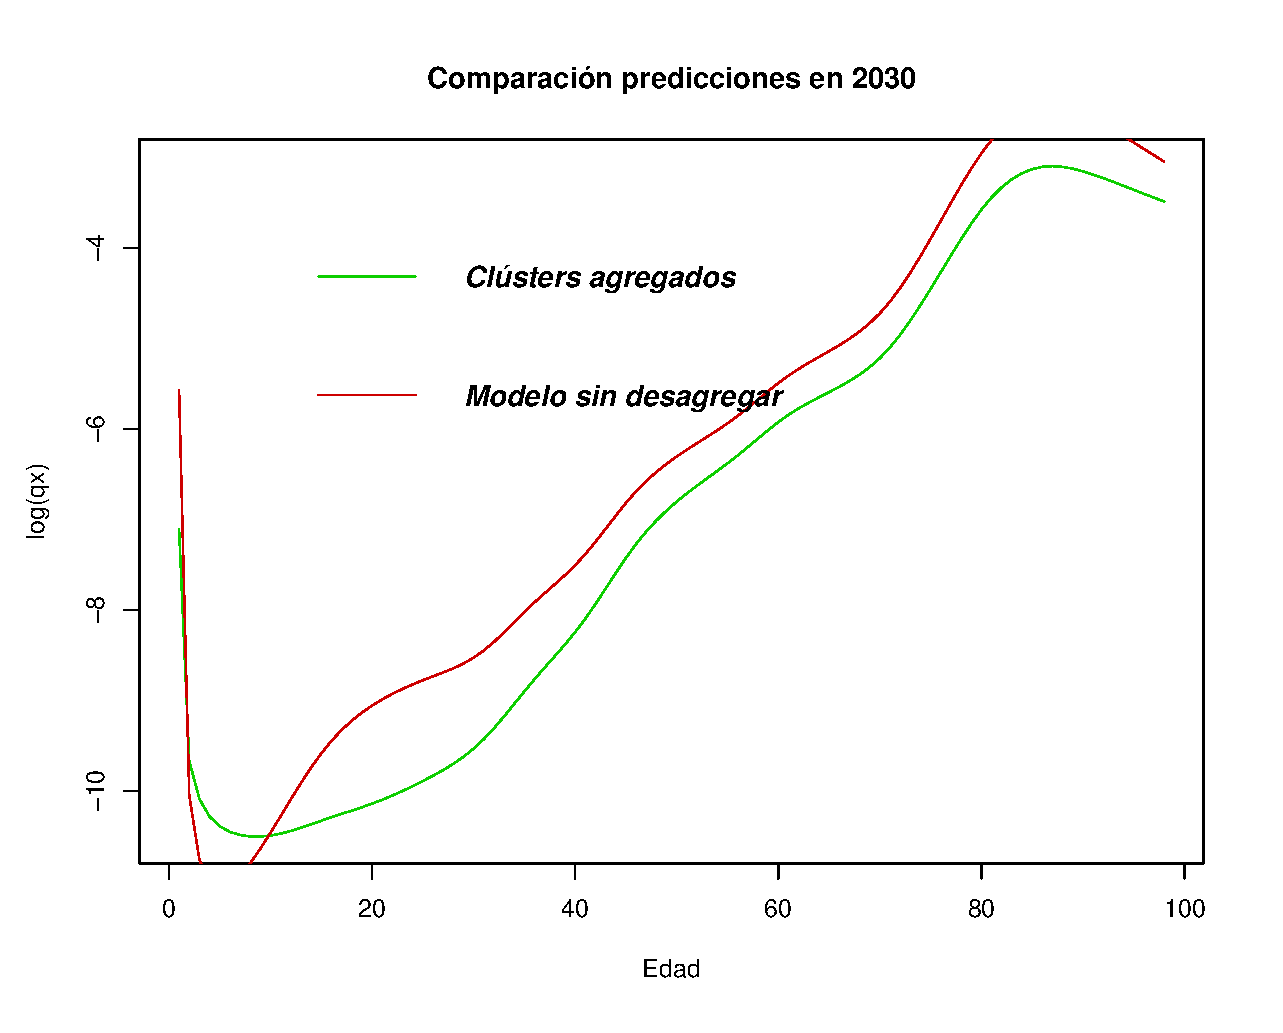
\includegraphics[width=0.55\textwidth]{comp30.eps}}
\caption{\centering Comparación de las predicciones de la mortalidad total. \\ \textbf{Fuente:} Elaboración propia.}
\label{comparaciontotal}
\end{figure}



Se concluye así que la desagregación de las causas para la predicción de la mortalidad es un método de estabilización de las predicciones a largo plazo, siendo las agrupaciones las encontradas a partir de distintos algoritmos de clustering para la similitud de evoluciones y los modelos utilizados para la modelización los clásicos modelos de mortalidad de Lee-Carter.

Para finalizar el apartado de resultados, se ha realizado el cálculo de las esperanzas de vida condicionadas a los grupos de causas de mortalidad creados, con los que se podrá predecir su futura evolución.

\subsection{Esperanzas de vida condicionadas}

En cuanto a la esperanza de vida al nacer, se ha obtenido la esperanza de vida cada conjunto de causas siguiendo los razonamientos de la nomenclatura tratada al inicio de este trabajo, en la que se indica cómo calcular la esperanza de vida respecto a un conjunto de causas, que se interpreta como los años esperados a vivir siendo el fallecimiento provocado por alguna de las causas incluídas en el cluster. Los resultados obtenidos son los que siguen:

\begin{table}[H]
\centering
   \label{espclust}
\begin{tabular}{c|cccc}
Año & Cluster 1 & Cluster 2 & Cluster 3 & Cluster 4 \\ 
  \hline
2015 & 698.60 & 91.61 & 103.47 & 518.77 \\ 
  2016 & 695.46 & 91.80 & 104.25 & 540.88 \\ 
  2017 & 692.34 & 92.00 & 105.04 & 564.10 \\ 
  2018 & 689.23 & 92.20 & 105.84 & 588.47 \\ 
  2019 & 686.14 & 92.40 & 106.66 & 614.06 \\ 
  2020 & 683.06 & 92.60 & 107.50 & 640.93 \\ 
  2021 & 680.00 & 92.80 & 108.35 & 669.14 \\ 
  2022 & 676.96 & 93.01 & 109.22 & 698.76 \\ 
  2023 & 673.92 & 93.22 & 110.11 & 729.86 \\ 
  2024 & 670.91 & 93.43 & 111.02 & 762.52 \\ 
  2025 & 667.91 & 93.64 & 111.94 & 796.81 \\ 
  2026 & 664.92 & 93.86 & 112.89 & 832.82 \\ 
  2027 & 661.95 & 94.07 & 113.85 & 870.63 \\ 
  2028 & 658.99 & 94.29 & 114.84 & 910.33 \\ 
  2029 & 656.05 & 94.52 & 115.85 & 952.01 \\ 
  2030 & 653.12 & 94.74 & 116.88 & 995.78 \\ 
  2031 & 650.21 & 94.97 & 117.93 & 1041.75 \\ 
  2032 & 647.31 & 95.20 & 119.00 & 1090.00 \\ 
  2033 & 644.42 & 95.43 & 120.10 & 1140.67 \\ 
  2034 & 641.55 & 95.67 & 121.22 & 1193.87 \\ 
  2035 & 638.70 & 95.91 & 122.37 & 1249.73 \\ 
\vdots &\vdots &\vdots &\vdots &\vdots \\
  2055 & 584.48 & 101.40 & 151.72 & 3177.37 \\ 
  2056 & 581.91 & 101.72 & 153.57 & 3330.43 \\ 
  2057 & 579.35 & 102.04 & 155.47 & 3490.80 \\ 
  2058 & 576.81 & 102.36 & 157.42 & 3658.78 \\ 
  2059 & 574.28 & 102.69 & 159.41 & 3834.70 \\ 
  2060 & 571.76 & 103.03 & 161.45 & 4018.87 \\ 
  2061 & 569.25 & 103.37 & 163.54 & 4211.65 \\ 
  2062 & 566.76 & 103.71 & 165.68 & 4413.36 \\ 
  2063 & 564.28 & 104.06 & 167.88 & 4624.34 \\ 
  2064 & 561.81 & 104.41 & 170.12 & 4844.94 \\ 
\end{tabular}
\caption{\centering Esperanzas de vida condicionadas a las muertes de cada cluster. \\ \textbf{Fuente:} Elaboración propia.}
\label{tablaesper}
\end{table}

Destacar inicialmente que la esperanza al nacer en cada cluster es superior a la esperanza de vida que se conoce comúnmente, llegando a ser para el cluster 1 y 4 superiores a 500 años. Esto viene dado debido a que la esperanza de vida que aquí se considera es la estudiada en el apartado 2.4, y que no incluye la posibilidad de fallecer por todas las causas, por lo que al tener menos tasas de fallecimiento disminuyendo su resultado, su valor incrementa. Esto explica el significado de los grandes valores obtenidos para los clusters 1 y 4, que son clusters con una y dos causas respectivamente, a parte de no ser causas con una gran cantidad de fallecimientos (figura \ref{distrclust}), por lo que fallecer por alguna de estas causas exclusivamente sin tener en cuenta las demás provoca esperanzas de vida de tal calibre.
Esta tabla se puede interpretar mejor si se plotea:

\begin{figure}[H]
\centering
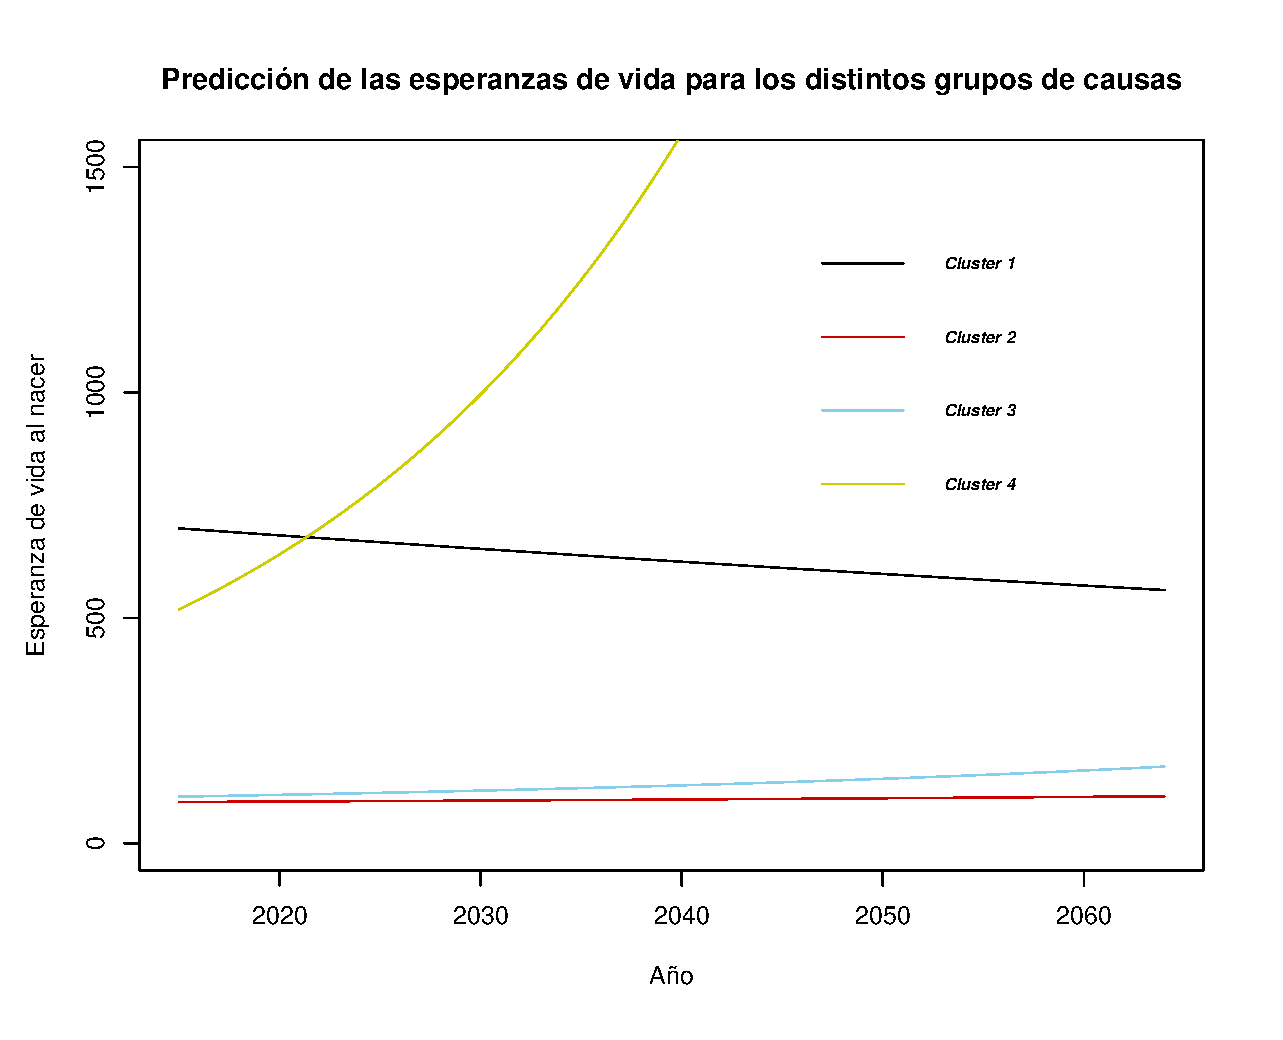
\includegraphics[scale=0.6]{esperclust.eps}
\caption{\centering Predicción de las esperanzas de vida al nacer para los cuatro clusters. \\ \textbf{Fuente:} Elaboración propia.}
\label{esperevo}
\end{figure}

La figura \ref{esperevo} indica distintas conclusiones importantes. Primero destaca el fuerte crecimiento que tiene el cluster 4, cluster que contiene las causas de fallecimiento \emph{embarazo, parto y puerperio} y \emph{síntomas, signos y hallazgos anormales clínicos y de laboratorio}. Este crecimiento predice claramente una disminución de la mortalidad por estas dos causas. Por otra parte, con un crecimiento más atenuado, aparecen las esperanzas de vida al nacer de los clusters 2 y 3, donde se encuentran la gran mayoría de las causas (ver cuadro \ref{causmean}). Este ligero crecimiento, siendo más acentuado para el cluster 3, indica que las causas incluidas en los clusters 2 y 3 van a disminuir sus respectivas tasas de mortalidad a lo largo de los años. Finalmente destacar que el cluster 1, cluster que sólo incluye la causa \emph{enfermedades infecciosas y parasitarias}, presenta un acentuado decrecimiento, lo que es un claro síntoma de que se prevee un crecimiento de los fallecimientos por esta causa.

\vspace{0.3cm}

\newpage
\section{Conclusiones}

Se detallarán ahora las conclusiones a las que se han llegado a partir del trabajo realizado y expuesto anteriormente.

\vspace{0.3cm}

A partir de la figura \ref{qxtot} se aprecia la evolución de la mortalidad total en España desde 1987 hasta 2014, en la que se ha observado cómo ha ido reduciéndose a lo largo de los años para todos los grupos de edad excepto en los 90 para las edades comprendidas entre los 20 y los 40 años, lo que fue provocado por el aumento de accidentes y enfermedades de transmisión sexual en estos años. Se han obtenido a partir del INE las defunciones por causas de mortalidad para poder modelizarlas por separado. Debido a que algunas causas presentan pocos fallecimientos y se producirían inconsistencias en los modelos (figura \ref{distrcaus}), se ha decidido agrupar las causas de mortalidad a partir de algorítmos de clustering siguiendo su evolución histórica para que su predicción futura sea consistente, finalmente en 4 clusters, lo cual ha sido razonado a partir de las siluetas medias producidas en el cuadro \ref{siluetas} y distintos algoritmos de clustering jerárquico (figuras \ref{dendr1}, \ref{dendr2} y \ref{dendr3}). La organización final de las causas queda reflejada en el cuadro \ref{nomclust}, en el que se observa qué causa pertenece a cada una de las agrupaciones realizadas. En la figura \ref{clustevol} se pueden observar qué causas provocan las tendencias de cada parte de la curva de mortalidad, siendo el cluster 3 el causante de la joroba social, y es en la figura \ref{clustevotime} donde se observa como son las edades más tempranas las que han presentado una mayor variabilidad a lo largo de los años.

\vspace{0.3cm}

A continuación, se han mostrado los parámetros obtenidos para los modelos de Lee-Carter de cada uno de los ajustes. Al representar estos parámetros se ha concluido que los factores representativos en los clusters 1, 2 y 3 son los que indican el decrecimiento en respuesta a los cambios y la variación del tiempo, y para el cluster 4, son los índices de variación en el tiempo del nivel de mortalidad (figuras \ref{params12} y \ref{params34}). 

\vspace{0.3cm}

Respecto a la predicción que se ha obtenido con el modelo agregado y con el modelo sin agregar, se puede observar en la figura \ref{prediction2015} la alta precisión obtenida por ambos modelos y, debido a que no queda claro qué modelo ajusta con mayor precisión, se ha decidido presentar en la figura \ref{comparaciontotal} las predicciones a largo plazo de ambos modelos, lo que nos indica que el modelo desagregado por clusters produce una mayor estabilidad en predicciones futuras, por tanto el separar por clusters para predecir la mortalidad total es una mejor herramienta de predicción debido a su estabilidad futura.

\vspace{0.3cm}

Finalmente se ha querido hacer mención a las esperanzas de vida condicionadas a los grupos de causas creados, en los que se observa a partir de la figura \ref{esperevo} cómo el cluster 4 presenta un acentuado aumento en su esperanza de vida al nacer, por lo que se espera una reducción de los fallecimientos por las causas incluídas en tal cluster (ver tabla \ref{nomclust}). Con crecimiento pero menos acentuado se encuentran las causas de los clusters 2 y 3, por lo que se espera que estas causas vayan reduciendo ligeramente su mortalidad a partir de las predicciones realizadas. Totalmente al contrario ocurre para el cluster 1, donde la esperanza de vida condicionada a la única causa que incluye (\emph{enfermedades infecciosas y parasitarias}) disminuye, lo que indica un aumento de las defunciones por esta causa.

\vspace{0.3cm}

Sólo queda realizar tres recomendaciones para poder incidir más en este tema. La primera es tener en cuenta la causa de mortalidad \emph{enfermedades infecciosas y parasitarias} ya que se ha predecido un gran aumento de su presencia para el futuro. La segunda es que los datos tomados del INE están agrupados por grupos de edad de 5 años, y como bien se sabe, el modelo de Lee-Carter producirá un mejor ajuste si se pudiesen obtener tales datos, aunque con estas agrupaciones de edad se ha podido demostrar la consistencia del ajuste y la razón principal del trabajo. La tercera y última es la fácil inclusión de la proporción de mortalidad de una defunción a cada una de las causas, ya que no sería un problema el incluir el porcentaje asociado de una muerte a una causa, y a partir de estos datos y los razonamientos del apartado 2.3 se podría realizar un estudio más exhaustivo de la mortalidad española, que tan útil es para la sociedad.



\vspace{0.3cm}

Cada día tomar datos es más sencillo y, junto a la algoritmos estadísticos que se poseen en la actualidad, cada día es más fácil predecir el futuro.

\newpage
\includepdf[pages={1,2,3}]{cie10.pdf}

\newpage
\bibliographystyle{habbrvyr}
\bibliography{TFM.bib}
\nocite{*}





\end{document}